\newif\ifbaskerville \baskervilletrue

\newif\ifpictures \picturesfalse

\documentclass[a4paper,11pt]{article}
\ifbaskerville
%% \usepackage{gill-sans,newbaskerville}
%% \renewcommand{\sfdefault}{gill-sans}
\fi

% \usepackage{librebaskerville}
% \usepackage[T1]{fontenc}
\usepackage[T1]{fontenc}
\usepackage{fbb}
% \usepackage{hyperref}

\usepackage{incgraph,tikz}

\usepackage{xcolor}
\usepackage{graphicx}
\usepackage[utf8]{inputenc}
\usepackage{enumitem} \setdescription{noitemsep}

\DeclareUnicodeCharacter{00A0}{~}
\setlength{\topmargin}{-2.5cm}
\setlength{\textheight}{26.5cm}
\setlength{\oddsidemargin}{-5mm}
\setlength{\textwidth}{17cm}

%\makeatletter
%\def\@oddfoot{\reset@font\sffamily\hfil\thepage\hfil}
%\let\@evenfoot\@oddfoot
%\makeatother

\newcommand{\header}[4]{{\noindent \makebox[2cm][l]{#1} \hfill #2
    \hfill \makebox[2cm][r]{#3\hspace{-1mm}} \vspace{-1ex} \\ \rule{\textwidth}{1pt}
    \begin{center} \Large\sffamily\bfseries #4 \end{center}} \vspace{5ex}}

\newcommand{\weekday}[1]{\begin{flushleft}\bfseries #1 \end{flushleft}} %\medskip}
% \newcommand{\weekday}[1]{\medskip}
\newcommand{\closeday}{}
\newcommand{\overview}[3]
{\noindent \makebox[17cm][l]{#2\dotfill page~#3} \\}
% {\noindent \makebox[3.5cm][l]{#1}\makebox[12cm][l]{#2} page~#3 \\}

\newcommand{\emptysession}[2]
{\noindent \colorbox{gray!30}{\makebox[2.5cm][c]{#1}\hspace{3mm}%
\makebox[13.9cm][l]{\bfseries #2}} \medskip \\}
\newcommand{\session}[2]
{\noindent \colorbox{gray!30}{\makebox[2.5cm][c]{#1}\hspace{3mm}%
\makebox[13.9cm][l]{\bfseries #2}} \medskip \\
\noindent\begin{tabular}{@{~~~}cp{15cm}}}
\newcommand\chair[1]{\small\mdseries\hfill Chair: #1}
\newcommand{\slot}[2]{#1 & #2 \\}
\newcommand{\slotnumbered}[3]{\slot{#1}{#2 [\##3]}}
\newcommand{\authors}[1]{\multicolumn{2}{@{\hspace{2cm}}p{14.5cm}}{#1} \\}
\newcommand{\tutorialauthors}[1]{\multicolumn{2}{@{\hspace{3cm}}p{13.5cm}}{#1} \\}
\newcommand{\closesession}{\end{tabular} \bigskip \\}
\let\author=\textit

\ifpictures
\newcommand{\outputmap}{\includegraphics[width=\textwidth]{social-map.png}}
\else
\newcommand{\outputmap}{\bigskip (For a location map, see the inside back cover.)}
\fi

\begin{document}


% \incgraph[documentpaper, overlay={\node[red] at (page.center) {\Huge Picture sized to paper};}]
\incgraph[documentpaper][width=\paperwidth,height=\paperheight]{img/cover.png}


\header{POPL 2018}{Omni Hotel}{2018/01/07 -- 2018/01/13}{Overview}

\overview{}{Message from the Chairs}{\pageref{Preface}}

\overview{}{AEC Chairs' Report}{\pageref{aec}}

%\smallskip
\overview{}{Committees}{\pageref{Committees}}

%\ifpictures
%\smallskip
%\overview{}{Floorplan}{\pageref{Floorplan}}
%\fi

%\smallskip
\overview{}{Keynotes}{\pageref{Keynotes}}

%\smallskip
\overview{Evenings}{Evening Events}{\pageref{Socials}}

%\smallskip
% \overview{Supporters}{Supporters and Sponsors}{\pageref{Supporters}}


\weekday{Sunday, 07 January}
\overview{19th International Conference on Verification, Model Checking, and Abstract Interpretation}{VMCAI Day -- 1}{\pageref{VMCAI-07}}
\closeday

\weekday{Monday, 08 January}
\overview{19th International Conference on Verification, Model Checking, and Abstract Interpretation}{VMCAI Day -- 2}{\pageref{VMCAI-08}}
\overview{— ACM SIGPLAN Workshop on Partial Evaluation and Program Manipulation}{PEPM Day -- 1}{\pageref{PEPM-08}}
\overview{20th International Symposium on  Practical Aspects of Declarative Languages }{PADL Day -- 1}{\pageref{PADL-08}}
\overview{CPP 2018 - The 7th ACM SIGPLAN International Conference on Certified Programs and Proofs}{CPP Day -- 1}{\pageref{CPP-08}}
\overview{TutorialFest}{TutorialFest}{\pageref{TutorialFest-08}}
\closeday

\weekday{Tuesday, 09 January}
\overview{19th International Conference on Verification, Model Checking, and Abstract Interpretation}{VMCAI Day -- 3}{\pageref{VMCAI-09}}
\overview{— ACM SIGPLAN Workshop on Partial Evaluation and Program Manipulation}{PEPM Day -- 2}{\pageref{PEPM-09}}
\overview{20th International Symposium on  Practical Aspects of Declarative Languages }{PADL Day -- 2}{\pageref{PADL-09}}
\overview{CPP 2018 - The 7th ACM SIGPLAN International Conference on Certified Programs and Proofs}{CPP Day -- 2}{\pageref{CPP-09}}
\overview{NetPL 2018}{NetPL}{\pageref{NetPL-09}}
\overview{Probabilistic Programming Languages, Semantics, and Systems (PPS 2018)}{PPS}{\pageref{PPS-09}}
\overview{Programming Languages Mentoring Workshop}{PLMW}{\pageref{PLMW-09}}
\closeday

\weekday{Wednesday, 10 January}
\overview{Research Papers}{POPL Day -- 1}{\pageref{POPL-10}}
\closeday

\weekday{Thursday, 11 January}
\overview{Research Papers}{POPL Day -- 2}{\pageref{POPL-11}}
\overview{Student Research Competition}{SRC}{\pageref{SRC-11}}
\closeday

\weekday{Friday, 12 January}
\overview{Research Papers}{POPL Day -- 3}{\pageref{POPL-12}}
\closeday

\weekday{Saturday, 13 January}
\overview{The Fourth International Workshop on Coq for Programming Languages}{CoqPL}{\pageref{CoqPL-13}}
\overview{Off the Beaten Track 2018}{OBT}{\pageref{OBT-13}}
\overview{Principles of Secure Compilation}{PriSC}{\pageref{PriSC-13}}
\closeday

\newpage


\header{Preface}{}{}{Message from the Chairs}
\label{Preface}


\newcommand\person[1]{{#1}}
%\newcommand\person[1]{\emph{#1}}

\noindent

Welcome to POPL 2019, the
\emph{46\textsuperscript{th} ACM SIGPLAN Symposium
on the Principles of Programming Languages}.
%
POPL is a premier forum for the discussion of all aspects
of programming languages and programming systems, welcoming
both theoretical and experimental work on a wide variety of
topics, with an emphasis on work that is principled and enduring.
%
We hope that you will enjoy the proceedings,
including both the talks covering a wide range
of technical topics as well as the ``hallway track''
that presents opportunities for learning from
and interacting with researchers, developers,
and students across the planet.

%%% BEGIN:ANDREW

\paragraph{Technical Program}
%
There were 267 reviewed submissions to POPL 2019.
%
A program committee comprising 52 experts,
aided by 114 external reviewers, did the hard work of
thoughtfully evaluating these submissions.
%
Ultimately the program committee selected 77 papers (29\%)
to be presented at the conference and to appear in the
proceedings. 
%
The program is also augmented by three journal papers that were accepted to
the ACM Transactions on Programming Languages and Systems (TOPLAS) during
2018.
%
Finally, the program also includes two invited keynotes by Mark Harman
and Brigitte Pientka.

All papers accepted for POPL 2019 are being published as an issue of the new
journal, Proceedings of the ACM on Programming Languages (PACMPL), a Gold Open
Access journal publishing research on all aspects of programming languages,
from design to implementation and from mathematical formalisms to empirical
studies.

\paragraph{Distinguished Paper Award}

A new addition to POPL 2019 is the introduction of a ``Distinguished Paper
Award.'' This award highlights papers that the POPL program committee thinks
should be read by a broad audience due to their relevance, originality,
significance and clarity. At most 10\% of the accepted papers of POPL are
eligible for this distinction.

We are happy to announce that the distinguished papers of POPL 2019 are:

\begin{itemize}
\item {\em A Domain Theory for Statistical Probabilistic Programming}, by 
Matthijs Vákár, Ohad Kammar, and Sam Staton
\item {\em Gradual Parametricity, Revisited}, by
Matías Toro, Elizabeth Labrada, and Éric Tanter
\item {\em Structuring the Synthesis of Heap-Manipulating Programs}, by 
Nadia Polikarpova and Ilya Sergey
\item {\em From Fine- to Coarse-Grained Dynamic Information Flow Control and
    Back}, by
Marco Vassena, Alejandro Russo, Deepak Garg, Vineet Rajani, and Deian Stefan
\item {\em $A^2$ I: Abstract$^2$ Interpretation}, by 
Patrick Cousot, Roberto Giacobazzi, and Francesco Ranzato
\item {\em Context-, Flow- and Field-Sensitive Data-Flow Analysis using
  Synchronized Pushdown Systems}, by
Johannes Späth, Karim Ali, and Eric Bodden
\end{itemize}

The selection of the distinguished papers was made based on the final versions
of the papers and through a second review process. The Distinguish Paper Award
committee was drawn from the POPL program committee and includes Andreas Abel,
Michael Greenberg, Suresh Jagannathan, Peter O'Hearn, Andrew Tolmach, and
Stephanie Weirich (chair).

\paragraph{Reviewing Process}
%
The reviewing process for POPL 2019 followed the guidelines laid out in
``Principles of POPL'' (Dreyer et al), making no major changes to the process
used by POPL 2018. After the reviewing process was complete, the PC members
were polled about their experience and all PC members responded except for one
member who left the PC due to personal reasons.

Key features of the POPL review process include:
\begin{itemize}
\item Lightweight double-blind submission: Reviews were written without
  exposing authorship to reviewers until the discussion phase.
\item Automated paper assignment: PC members had the option of identifying a
  small number of papers they were genuinely interested in reviewing. The
  remainder of their reviewing assignments were done using the Toronto Paper
  Matching System (TPMS), an unsupervised machine learning algorithm supported
  by Laurent Charlin. The overall response of the PC was that their assigned
  papers were at least as well to their expertise as in previous conference
  reviewing and less work was required from PC members.
\item Two-phase reviewing: Papers were initialially assigned two PC reviewers
  and only allocated additional reviews if the first two reviews were
  positive. In the post-PC poll, 41 PC members found the multiple rounds
  useful, whereas 3 reported that it did not work well.
\item Author response: All authors were given the chance to respond to their
  reviews before the PC discussion period. In the post-PC poll, 40 PC members
  reported that the author response had a positive effect on decisions and
  reviews and 2 reported a negative effect.
\item Online PC meeting: Paper discussions were conducted electronically,
  primarily using the excellent HotCRP system developed and supported by Eddie
  Kohler. (More details below.)
\item Conflicts: PC members were allowed to submit and all conflicts were
  managed by the HotCRP system. PC papers were marked in the system and held
  to a higher standard than non-PC authored papers. Chair conflicts were
  managed by Lars Birkedal, who will be the PC chair for POPL 2020.
\item Conditional acceptance: Due to publication in PACMPL, all papers were
  conditionally accepted and any changes by the authors were reviewed prior to
  publication. Each conditionally accepted paper was assigned a ``shepherd''
  from the PC, who worked with the authors and reviewers to ensure that
  reviewer feedback was addressed by the final version of every paper. Every
  conditionally accepted paper was eventually revised to the satisfaction of
  the reviewers.
\end{itemize}

Following the practice initiated by POPL 2018, all discussion of papers took
place online. The rationale for this change was that while physical meetings
have real benefits, these benefits have not kept pace with the costs as POPL
has grown.  Having the entire PC fly to one spot on the globe for a two-day
meeting requires considerable time and energy from PC members, and the travel
comes with significant monetary and environmental cost.  While a face-to-face
meeting facilitates engaging discussions and strengthens the research
community, especially for junior members of the PC, these positive effects
have diminished as the PC has grown. Having no physical meeting made it
possible to invite a PC of more than 50 members. A larger PC both increases
the coverage of topics among the PC members and ensures that the reviewing
load for individual PC members is manageable.

Overall, the sentiment of the PC was to continue with this format, answering
the question ``Should we have online PC meetings in the future?'' with 31
answering ``yes'' and seven ``no''.  The PC members also commented in the poll
about the benefits of an online meeting, reiterating the rationale above and
also pointing out a few additional benefits. In particular, some commented
that they found the discussion to be more in depth and that it was easier to
make their opinions heard than in a physical meeting. They also appreciated
the asynchronous nature of the meeting, where decisions were not biased by a
discussion order and commented on the fact that an online meeting makes it
easier for PC members to easier to incorporate discussion into the feedback
for the authors.  The negative comments about the change included the
difficulty of keeping up with several discussions in parallel and the lack of
``global view'' of the program, making it difficult for them to identify
related papers to join in the discussion. In particular, some expressed
concern that the program would become more fragmented and less accessible to
the broader community.

There are concerns that an online discussion decreases the level engagement of
PC member, and the results of the poll were mixed. Equal numbers of PC members
found that that their engagement increased as well as decreased (12 each way),
while over half of the PC members reported no change. Furthermore, when asked
whether the online discussion made it easier or harder to follow the
arguments, 27 members reported a positive effect and 8 members reported a
negative effect.  Similarly, PC members thought that the online meeting helped
the review quality: 26 members thought that reviews were improved by this
format and only three thought that that they were negatively affected.

\paragraph{Affiliated Events}
%% FRITZ: check this I just changed the dates and numbers
%
We are very pleased that POPL 2019 continues the tradition of being enriched
by a host of co-located events.
%
These include three co-located conferences,
%
\begin{itemize}
  \item CPP 2019:   The \emph{8\textsuperscript{th} ACM SIGPLAN Intl. Conference on Certified Programs and Proofs},
  \item PADL 2019:  The \emph{21\textsuperscript{th} Intl. Symposium on Practical Aspects of Declarative Languages}, and
  \item VMCAI 2019: The \emph{20\textsuperscript{th} Intl. Conference on Verification, Model Checking, and Abstract Interpretation}.
\end{itemize}
%
Seven colocated workshops focus on variety of foundational and applied topics,
%
\begin{itemize}
  \item CoqPL 2019: \emph{The 5\textsuperscript{th} Intl. Workshop on Coq for Programming Languages},
  \item NetPL 2019: \emph{The 5\textsuperscript{th} Intl. Workshop on Networking and Programming Languages},
  \item PEPM 2019:  \emph{The ACM SIGPLAN Workshop on Partial Evaluation and Program Manipulation}
  \item OBT 2019:   \emph{Off the Beaten Track}
  \item PriSC 2019: \emph{Principles of Secure Compilation}
  \item PPS 2019:   \emph{Probabilistic Programming Languages, Semantics, and Systems},
\end{itemize}
%
Finally, we are especially happy about two events that
focus on inspiring senior undergraduate and beginning
graduate students to pursue programming languages and
that aim to help them become a part of the research
community.
%
\begin{itemize}
\item SRC: \emph{Student Research Competition}, and
\item PLMW: \emph{Programming Languages Mentoring Workshop} at POPL.
\end{itemize}
%
All the above events have joint lunch and coffee breaks
and the same overall schedule structure so that registrants
at any event can attend talks at the other.

\paragraph{Thanks}
%%%fritz, please edit here
%
POPL has grown and thrived for 46 years primarily thanks to
the vibrant community that supports and sustains it.
%
This community includes the authors and developers who
provide the talks and posters, the attendees -- both local
as well as remote -- who provide a stimulating environment
for discussion and debate.
%
However, we would like to especially recognize the \emph{many}
volunteers who---despite their other onerous commitments---have
taken on new responsibilities to help put together this symposium.
%
We are immeasurably thankful for their dedication, effort and expertise.
%
In particular, we would like to thank
%
the program committee, the external reviewers,
and \person{Jean Yang} and \person{C\u{a}t\u{a}lin Hri\c{t}cu}
and the artifact evaluation committee for their
thorough and thoughtful reviews;
%
\person{Marco Gaboardi} for skilfully organizing
the fantastic TutorialFest and co-ordinating with
all the co-located events;
%
the members of the POPL steering committee --- especially the current
chair \person{Giuseppe Castagna} and new chair \person{Michael Hicks} ---
for their long term stewardship and dedication to the success
of the symposium;
%
\person{Jan Vitek} for being incredibly generous with his time,
helping us put together the website and for many helpful
suggestions;
%
\person{David Walker}, for liaising with our industrial
partners and arranging the generous support and
sponsorships that make POPL possible;
%
\person{Alexandra Silva}, \person{Steve Zdancewic},
\person{Nadia Polikarpova} and \person{Viktor Vafeiadis}
for organizing PLMW;
%
\person{Benjamin Delaware} for running the Student Research Competition;
%
\person{Jean Yang} and \person{Rohit Singh}, for their many novel innovations
using social media and the web to grow the POPL community and
keep it informed, including the wonderful new ``People of Programming Languages''
interviews;
%
\person{Michael Greenberg} for helping POPL transition into a remote participation
era, in which anyone on the planet can engage with the speakers even
if they couldn't be physically present in Los Angeles;
%
% CHECK: José Calderón for managing the process of recording and posting videos
% CHECK: for many of the talks at ICFP and associated events;
%
\person{Dirk Beyer} and Conference Publishing Consulting
for compiling the proceedings;
%
the PACMPL Editorial Board and the staff at ACM
headquarters---especially \person{Philip Wadler}---for guiding
and supporting the transition to PACMPL;
%
\person{Alex Sanchez-Stern} and \person{Jakub Zalewski} for organizing
and leading the team of student volunteers
working to keep everything running like clockwork;
%
\person{John Otero} at ACM for helping us find a sweet
venue in downtown Los Angeles.
%
Finally, we will be forever indebted to
\person{Annabel Satin} and \person{Marta Zampollo},
for being the real force behind the conference
(and other SIGPLAN events!), and for making the
task of organizing POPL 2019 miraculously pleasant.

\paragraph{Supporters}
%
POPL 2019 was made possible by our partners, supporters
and sponsors whose generosity helps the community grow
and thrive by making it possible to keep the cost of
registration affordable, and by providing support for
students who would not have been able to attend without
financial aid.
%
We are also very grateful for the generous support of
ACM and ACM SIGPLAN, including their commitment to
PACMPL's Gold Open Access policy, making high-quality,
peer-reviewed scientific research available without
restrictions on access or (re-)use.

\medskip
Welcome again to POPL 2019. We hope you learn new things,
have fun, meet old friends and colleagues, make new
ones, and go home inspired!

\begin{flushright}
\textit{Fritz Henglein, University of Copenhagen} \\
POPL 2019 General Chair
\medskip \\
\textit{Stephanie Weirich, University of Pennsylvania} \\
POPL 2019 Program Chair
\medskip \\
\end{flushright}




\newpage

\header{Committees}{}{}{Committees}
\label{Committees}

\def\namewidth{6cm}

\subsection*{\sffamily Organizing Committee}

\def\member#1#2{\item[#1:] #2}

\begin{description}[font=\mdseries\itshape]
\member{General Chair}{Fritz Henglein}
\member{Program Chair}{Stephanie Weirich}
\member{Local Arrangements Chair}{Vasco Vasconcelos}
\member{Associated Events Chairs}{Marco Gaboardi, Zachary Kincaid}
\member{Industrial Relations Chair}{David Walker}
\member{Artifact Evaluation Chairs}{Benjamin Delaware, Cătălin Hriţcu}
\member{Publicity Chair}{Michael Greenberg}
\member{PLMW Chairs}{Justin Hsu, Bernardo Toninho, Nobuko Yoshida, Steve Zdancewic}
\member{Student Research Competition Chair}{Niki Vazou}
\member{Web Chair}{Hsiang-Shang `Josh' Ko}
\member{Video Chair}{Jakub Zalewski}
\member{Student Volunteer Captains}{Carlos Mão de Ferro, Alex Sanchez-Stern}
\member{Conference Coordinator and Treasurer}{Annabel Satin}
\member{Registration}{Carole Mann}
\end{description}

\subsection*{\sffamily POPL Steering Committee}

\begin{tabular}{@{}p{\namewidth}l@{}}
Michael Hicks (Chair) & University of Maryland, USA \\
Jens Palsberg & University of California, Los Angeles, USA \\
Benjamin C. Pierce & University of Pennsylvania, USA \\
Giuseppe Castagna & CNRS/University of Paris Diderot, France \\
Brigitte Pientka & McGill University, Canada \\
David Walker  & Princeton University, USA \\
Jeremy Gibbons  & University of Oxford, UK \\
Andrew D. Gordon  & Microsoft Research/University of Edinburgh, UK \\
Ranjit Jhala  & University of California, San Diego, USA \\
Andrew Myers  & Cornell University, USA \\
Fritz Henglein & University of Copenhagen, Denmark \\
Stephanie Weirich & University of Pennsylvania, USA \\
Lars Birkedal & Aarhus University, Denmark \\
\end{tabular}

\subsection*{\sffamily Program Committee}

\begin{tabular}{@{}p{\namewidth}l@{}}
Andrew Myers (Chair)
  & Cornell University, USA  \\
Thorsten Altenkirch
  & University of Nottingham, UK \\
Nada Amin
  & University of Cambridge, UK \\
Gilles Barthe
  & IMDEA Software Institute, Spain \\
Mark Batty
  & University of Kent, UK \\
Lars Birkedal
  & Aarhus University, Denmark \\
Pavol Cerny
  & University of Colorado Boulder, USA \\
James Cheney
  & University of Edinburgh, UK \\
Koen Claessen
  & Chalmers University of Technology, Sweden \\
William Cook
  & University of Texas at Austin, USA \\
Karl Crary
  & Carnegie Mellon University, USA \\
Loris D'Antoni
  & University of Wisconsin–Madison, USA \\
Mila Dalla Preda
  & University of Verona, Italy \\
Isil Dillig
  & University of Texas at Austin, USA \\
Sophia Drossopoulou
  & Imperial College, UK \\
Constantin Enea
  & Université Paris Diderot, France \\
Azadeh Farzan
  & University of Toronto, Canada \\
Xinyu Feng
  & University of Science and Technology, China \\
Atsushi Igarashi
  & Kyoto University, Japan \\
Laura Kovacs
  & Chalmers University of Technology, Sweden \\
Neel R. Krishnaswami
  & University of Cambridge, UK \\
Sorin Lerner
  & University of California, San Diego, USA \\
Xavier Leroy
  & INRIA, France \\
Conor McBride
  & University of Strathclyde, UK \\
Mira Mezini
  & TU Darmstadt, Germany \\
Matthew Might
  & University of Utah, USA \\
Peter Müller
  & ETH Zurich, Switzerland \\
Santosh Nagarakatte
  & Rutgers University, USA \\
Aleksandar Nanevski
  & IMDEA Software Institute, Spain \\
Klaus Ostermann
  & University of Tuebingen, Germany \\
Ruzica Piskac
  & Yale University, USA \\
Nadia Polikarpova
  & University of California, San Diego, USA \\
Zvonimir Rakamaric
  & University of Utah, USA \\
Aseem Rastogi
  & Microsoft Research, India \\
Grigore Rosu
  & University of Illinois at Urbana-Champaign, USA\\
Andrey Rybalchenko
  & Microsoft Research, United Kingdom \\
Amr Sabry
  & Indiana University, USA \\
David Sands
  & Chalmers University of Technology, USA \\
Davide Sangiorgi
  & University of Bologna, Italy \\
Peter Sewell
  & University of Cambridge, UK \\
Zhong Shao
  & Yale University, USA \\
Yannis Smaragdakis
  & University of Athens, Greece \\
Zhendong Su
  & University of California, Davis, USA \\
Éric Tanter
  & University of Chile, Chile \\
Zachary Tatlock
  & University of Washington, USA \\
Tachio Terauchi
  & Waseda University, Japan \\
Viktor Vafeiadis
  & MPI-SWS, Germany \\
Philip Wadler
  & University of Edinburgh, UK \\
David Walker
  & Princeton University, USA \\
Stephanie Weirich
  & University of Pennsylvania, USA \\
Jean Yang
  & Carnegie Mellon University, USA \\
Danfeng Zhang
  & Pennsylvania State University, USA \\
\end{tabular}

\subsection*{\sffamily Additional Reviewers}

\begin{tabular}[t]{@{}p{\namewidth}}
Adam Chlipala
\\ Alceste Scalas
\\ Ales Bizjak
\\ Alex Kavvos
\\ Alex Summers
\\ Alexandra Silva
\\ Andrea Cerone
\\ Andreas Abel
\\ Andreas Rossberg
\\ Andrej Bauer
\\ Andrzej Filinski
\\ Anthony Vandikas
\\ Aquinas Hobor
\\ Arjun Guha
\\ Armin Biere
\\ Arthur Azevedo de Amorim
\\ Barret Zoph
\\ Boris Yakobowski
\\ Carsten Fuhs
\\ Caterina Urban
\\ Cesare Tinelli
\\ Charles Grellois
\\ Chen Ding
\\ Chengnian Sun
\\ Chris Hawblitzel
\\ Christopher Pulte
\\ Chung-Kil Hur
\\ Chung-chieh Shan
\\ Craig McLaughlin
\\ Dan Ghica
\\ Dave Clarke
\\ David Naumann
\\ Davide Ancona
\\ Derek Dreyer
\\ Dimitrios Vytiniotis
\\ Dominic Orchard
\\ Eijiro Sumii
\\ Eric Mercer
\\ Garrett Morris
\\ Giorgio Delzanno
\\ Hanru Jiang
\\ Hongjin Liang
\\ Igor Konnov
\\ Isaac Sheff
\end{tabular}%
\begin{tabular}[t]{p{\namewidth}}
   Isabella Mastroeni
\\ Jade Alglave
\\ James Noble
\\ Jean Pichon-Pharabod
\\ Joost-Pieter Katoen
\\ Joseph Tassarotti
\\ Justin Hsu
\\ Kasper Svendsen
\\ Kazushige Terui
\\ Keita Yokoyama
\\ Krishnendu Chatterjee
\\ Liang-Ting Chen
\\ Luis Caires
\\ Madan Musuvathi
\\ Makarius Wenzel
\\ Malgorzata Biernacka
\\ Malte Schwerhoff
\\ Marco Gaboardi
\\ Marco Paviotti
\\ Mark Baranowski
\\ Martin Abadi
\\ Martin Vechev
\\ Maryam Dabaghchian
\\ Matthew Flatt
\\ Matthew Fluet
\\ Matthew Hammer
\\ Matthew Parkinson
\\ Michael Bond
\\ Michael Emmi
\\ Michele Boreale
\\ Miltos Allamanis
\\ Ming Kawaguchi
\\ Naoki Kobayashi
\\ Nate Foster
\\ Neil Jones
\\ Noam Zeilberger
\\ Ohad Kammar
\\ Olivier Danvy
\\ Paul Levy
\\ Peixuan Li
\\ Peter Sestoft
\\ Phil Trinder
\\ Philipp Ruemmer
\end{tabular}%
\begin{tabular}[t]{p{\namewidth}}
   Pierre-Yves Strub
\\ Pietro Di Gianantonio
\\ Premkumar Devanbu
\\ Qirun Zhang
\\ Ramana Kumar
\\ Ranald Clouston
\\ Ranjit Jhala
\\ Rasmus Ejlers Møgelberg
\\ Rasmus Møgelberg
\\ Robert Rose
\\ Rupak Majumdar
\\ Ryan Beckett
\\ Sabine Glesner
\\ Sam Lindley
\\ Sam Staton
\\ Sam Tobin-Hochstadt
\\ Sebastian Burckhardt
\\ Sergio Mover
\\ Shachar Itzhaky
\\ Shaked Flur
\\ Shaobo He
\\ Simon Fowler
\\ Soumyadeep Ghosh
\\ Sriram Sankaranarayanan
\\ Steven Awodey
\\ Steven Ramsay
\\ Sukyoung Ryu
\\ Taro Sekiyama
\\ Tiark Rompf
\\ Tom Hirschowitz
\\ Tomas Petricek
\\ Tomofumi Yuki
\\ Torsten Grust
\\ Uday Bondhugula
\\ Ugo Dal Lago
\\ Valeria Vignudelli
\\ Vasco Vasconcelos
\\ Vijay Ganesh
\\ Wolfgang Ahrendt
\\ Xiangyu Zhang
\\ Yaron Minsky
\\ Yoichi Hirai
\\ Zhoulai Fu
\end{tabular}

\subsection*{\sffamily Artifact Evaluation Committee}

\begin{tabular}{@{}p{\namewidth}l@{}}
Benjamin Delaware (Co-Chair)
  & Purdue University, USA\\
C\u{a}t\u{a}lin Hri\c{t}cu (Co-Chair)
  & Inria Paris, France \\
Aleš Bizjak
  & Aarhus University, Denmark\\
Amin Timany
  & imec-DistriNet, KU Leuven, Belgium\\
Ankush Das
  & Carnegie Mellon University, USA\\
Arthur Azevedo de Amorim
  & Carnegie Mellon University, USA\\
Casper Bach Poulsen
  & Delft University of Technology, Netherlands\\
Caterina Urban
  & ETH Zurich, Switzerland\\
Christine Rizkallah
  & University of New South Wales, Australia\\
Christopher Pulte
  & University of Cambridge, UK\\
Daniel Dietsch
  & University of Freiburg, Germany\\
Daniel Patterson
  & Northeastern University, USA\\
David Swasey
  & MPI-SWS, Germany\\
Di Wang
  & Carnegie Mellon University, USA\\
Gregory Essertel
  & Purdue University, USA\\
He Zhu
  & Galois, Inc, USA\\
Jan Stolarek
  & University of Edinburgh, UK and Politechnika Łódzka, Poland\\
Jeehoon Kang
  & Seoul National University, South Korea\\
Jeevana Priya Inala
  & MIT, USA\\
Jennifer Paykin
  & Galois, Inc, USA\\
Jesper Cockx
  & Gothenburg University, Sweden\\
Jonathan Protzenko
  & Microsoft Research, Redmond, USA\\
Karl Palmskog
  & The University of Texas at Austin, USA\\
Maillard Kenji
  & ENS Paris and Inria Paris, France\\
Martin Bodin
  & Imperial College London, UK\\
Robert Rand
  & University of Maryland, College Park, USA\\
Samuel Drews
  & University of Wisconsin-Madison, USA\\
Sara Achour
  & MIT CSAIL, USA\\
Talia Ringer
  & University of Washington, USA\\
Taro Sekiyama
  & National Institute of Informatics, Japan\\
Thomas Sewell
  & Data61, Australia\\
William Mansky
  & University of Illinois at Chicago, USA
\end{tabular}


\newpage

\ifpictures \header{Floorplan}{}{}{Hotel Cascais Miragem}
\label{Floorplan}

\paragraph{Gallery}
\begin{center}
  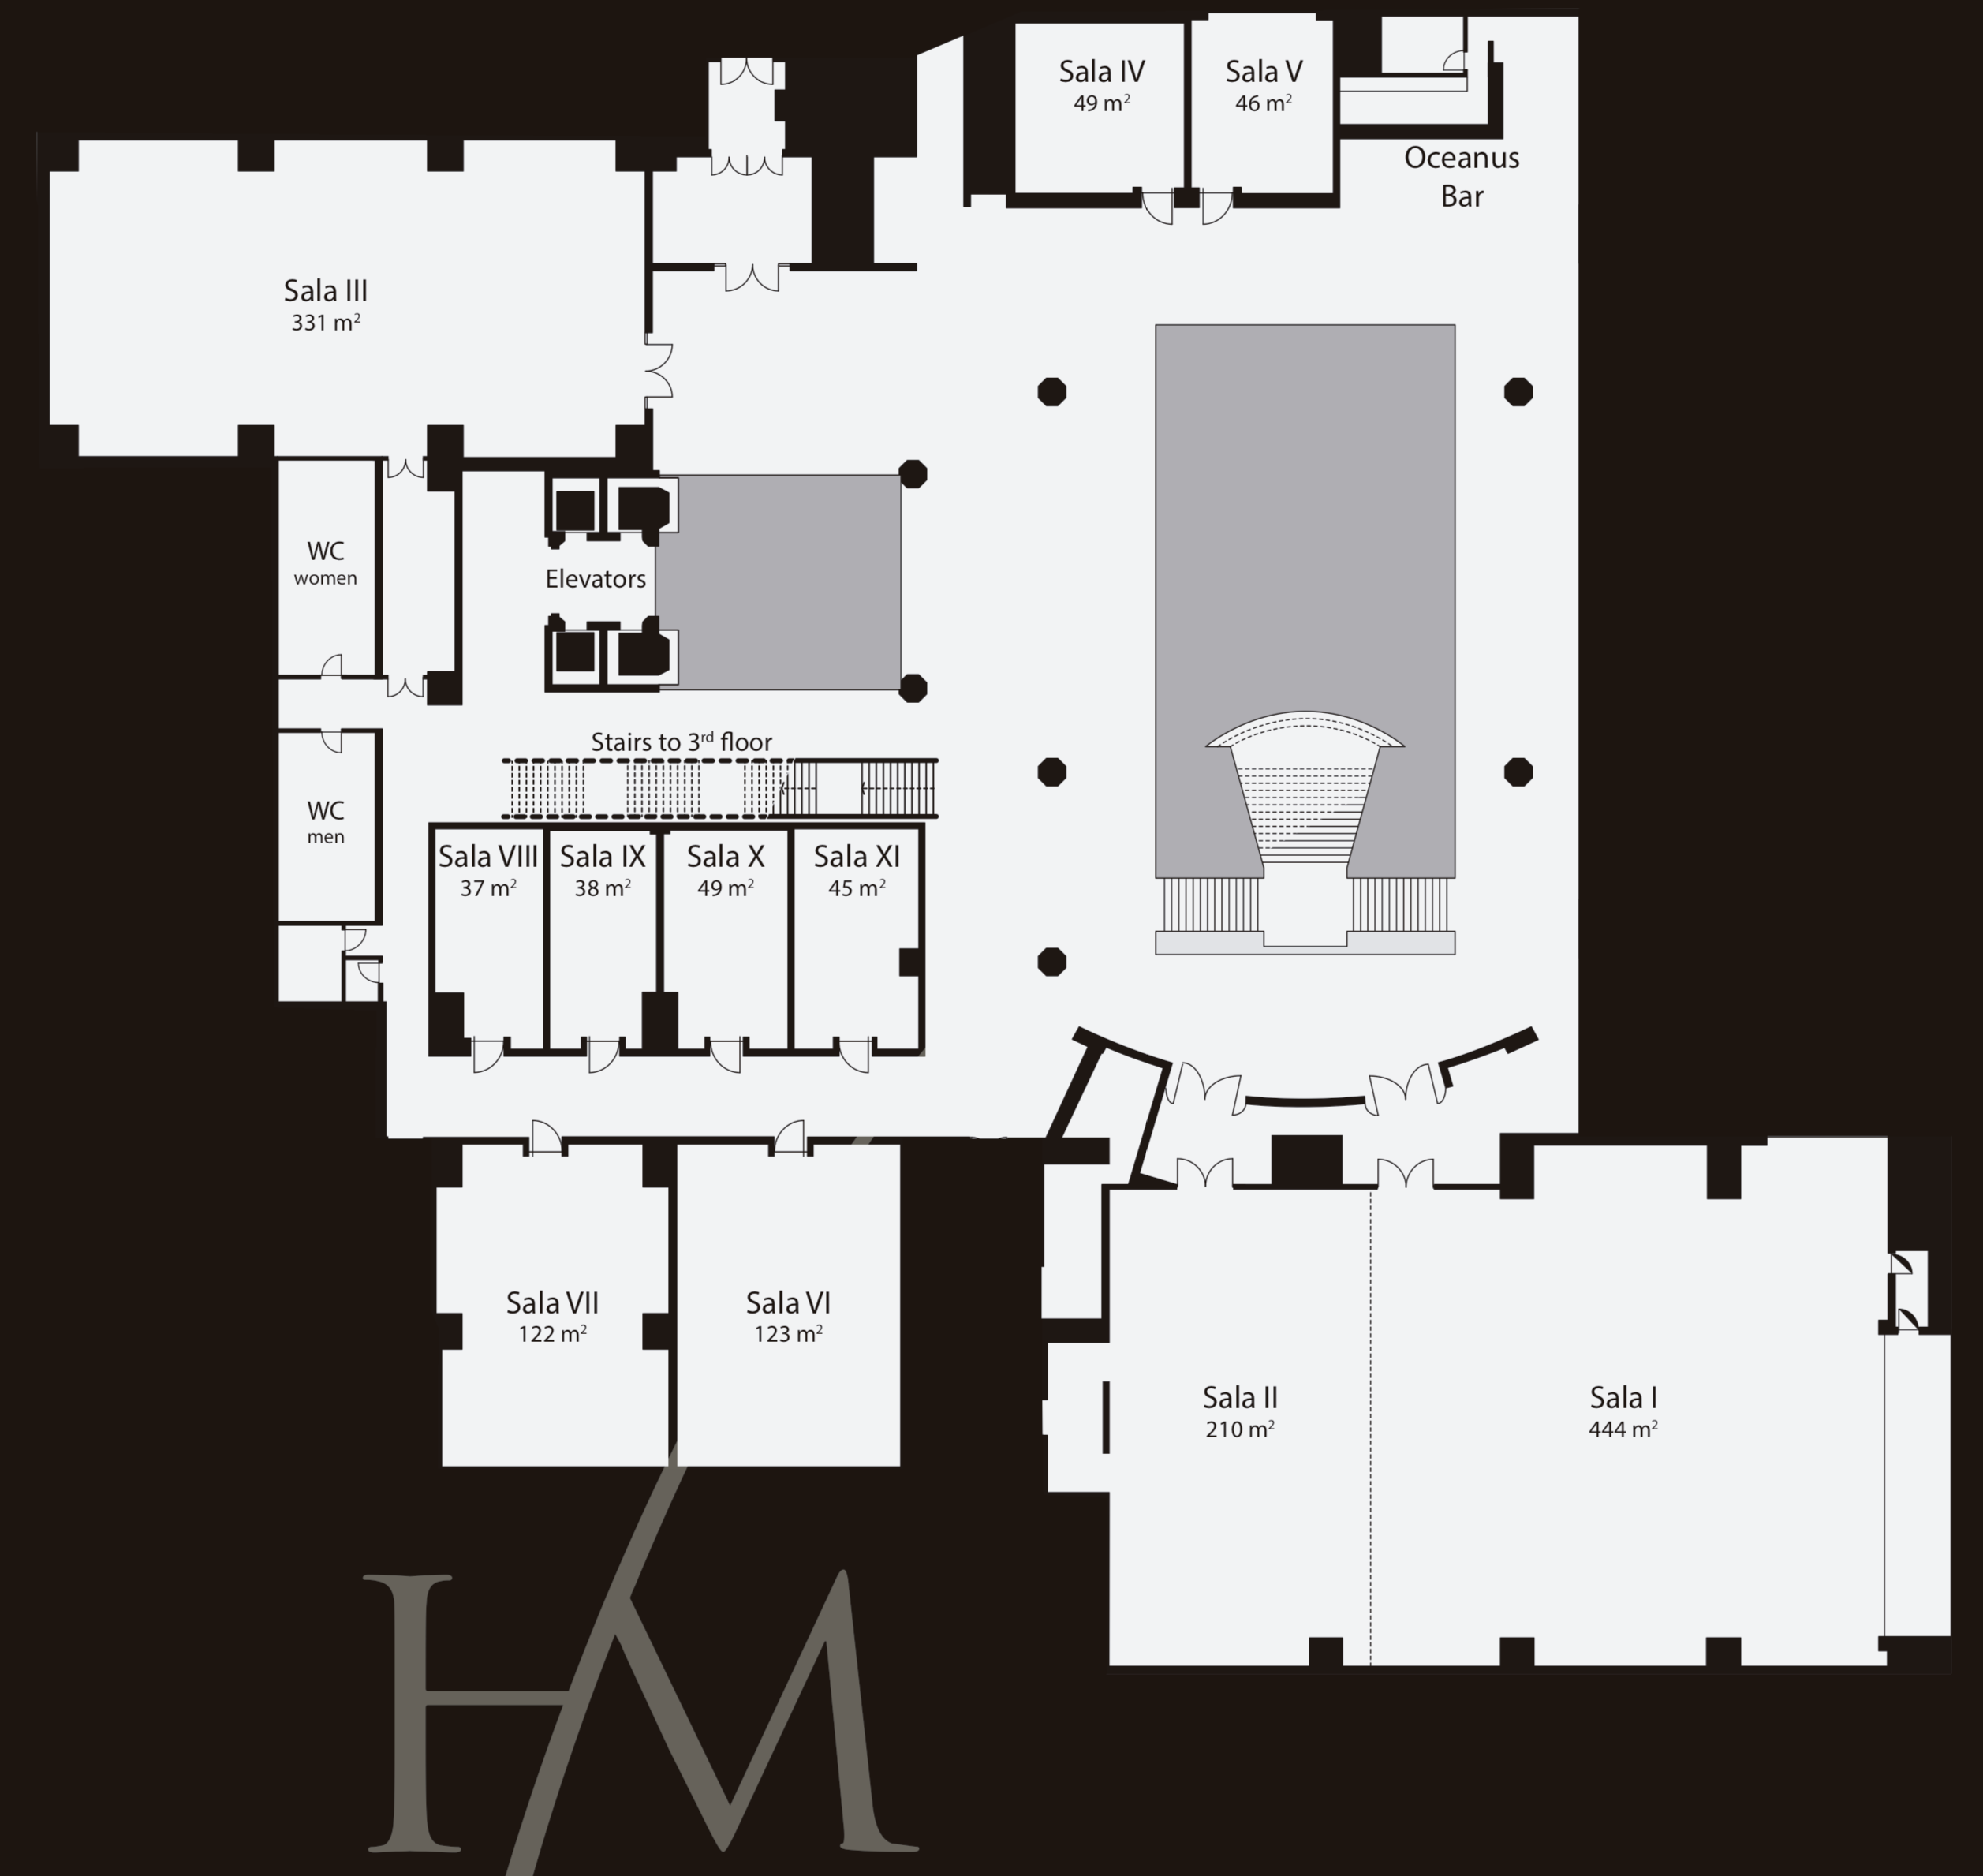
\includegraphics[width=0.7\textwidth]{img/gallery}
\end{center}

\paragraph{Lobby}
\begin{center}
  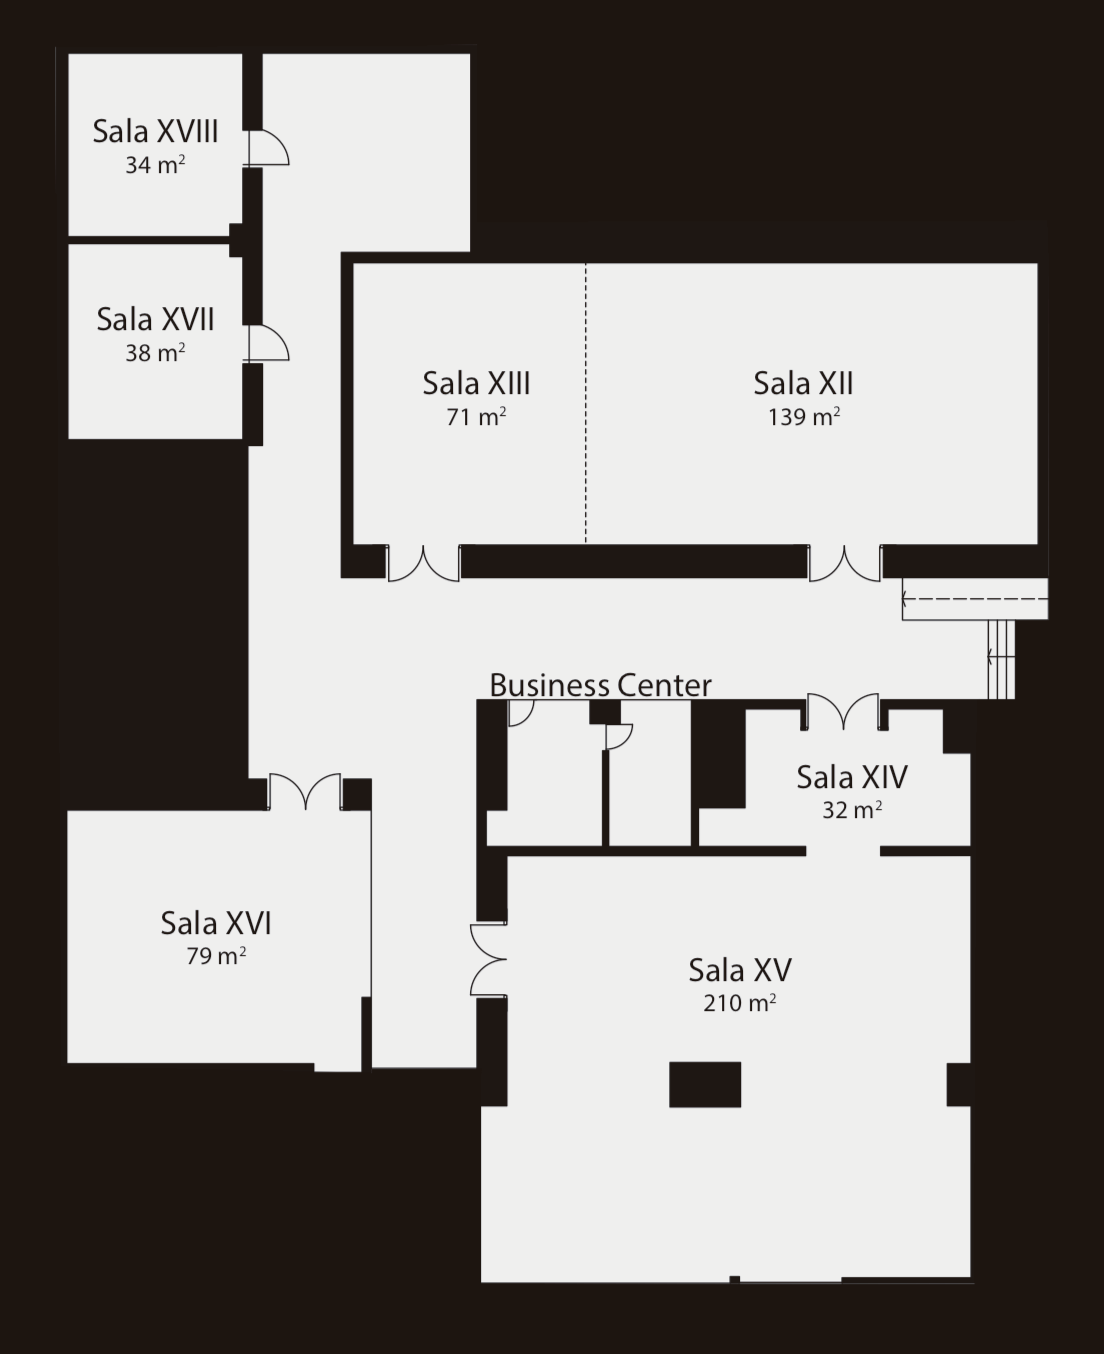
\includegraphics[width=0.35\textwidth]{img/lobby}
\end{center}

\vfil
\paragraph{WiFi}
\begin{description}
\item[SSID] \texttt{events}
\item[Password] \texttt{events2018}
\end{description}
% \begin{center}
% %\fbox{\Large\textbf{Wifi:} Connect to \textit{eduroam}, or sign up (for free) to \textit{The Cloud}.}
% \fbox{\Large\textbf{Wifi:} }
% \end{center}
\vfil
\eject

\newpage

%%% Local Variables:
%%% mode: latex
%%% TeX-master: t
%%% End:
 \fi
\header{Keynotes}{}{}{POPL Keynotes}
\label{Keynotes}

\def\talktitle#1{\subsection*{#1}}
\def\speaker#1#2{\begin{flushleft} #1 (#2) \end{flushleft}}
\def\talkabstract{\noindent \textbf{Abstract:}~}
\def\bio{\medskip\noindent \textbf{Bio:}~}

\talktitle{The Type Soundness Theorem That You Really Want to Prove (and Now You Can)}

\speaker{Derek Dreyer}{MPI-SWS}

\talkabstract
Type systems—and the associated concept of “type soundness”—are one of the
biggest success stories of foundational PL research. Originally proposed by
Robin Milner in 1978, type soundness asserts that well-typed programs can’t “go
wrong” (\emph{i.e.}, exhibit undefined behaviors), and it is widely viewed as the
canonical theorem one must prove to establish that a type system is doing its
job. In the early 1990s, Wright and Felleisen introduced a simple syntactic
approach to proving type soundness, which was subsequently popularized as the
method of ``progress and preservation'' and has had a huge impact on the study and
teaching of PL foundations. Many research papers that propose new type systems
conclude with a triumphant statement of syntactic type soundness, and for many
students it is the only thing they learn to prove about a type system.

Unfortunately, syntactic type soundness is a rather weak theorem. First of all,
its premise is too strong for many practical purposes. It only applies to
programs that are completely well-typed, and thus tells us nothing about the
many programs written in ``safe'' languages that make use of ``unsafe'' language
features. Even worse, it tells us nothing about whether type systems achieve one
of their main goals: enforcement of data abstraction. One can easily define a
language that enjoys syntactic soundness and yet fails to support even the most
basic modular reasoning principles for closures, objects, and ADTs.

In this talk, I argue that we should no longer be satisfied with just proving
syntactic type soundness, and should instead start proving a stronger
theorem—semantic type soundness—that captures more accurately what type systems
are actually good for. In a semantic soundness proof, one defines a semantic
model of types as predicates on values, and then verifies the soundness of
typing rules as lemmas about the model. By explaining directly what types
``mean'', the semantic approach to type soundness is a lot more informative than
the syntactic one. In particular, it can serve to establish what data
abstraction guarantees a language provides, as well as what it means for uses of
unsafe language features to be ``safely encapsulated''.

Semantic type soundness is a very old idea—Milner’s original formulation of type
soundness was a semantic one—but it fell out of favor in the 1990s due to
limitations and complexities of denotational models. In the succeeding decades,
such limitations have been overcome and complexities tamed, via proof techniques
that work directly over operational semantics. Thanks to the development of
step-indexed Kripke logical relations, we can now scale semantic soundness to
handle real languages, and thanks to advances in higher-order concurrent
separation logic, we can now build (machine-checked) semantic soundness proofs
at a much higher level of abstraction than was previously possible. The
resulting ``logical'' approach to semantic type soundness yields proofs that are
demonstrably more useful than their syntactic counterparts, and more fun as
well.

\bio
Derek Dreyer is a professor of computer science at the Max Planck Institute for
Software Systems (MPI-SWS), and recipient of the 2017 ACM SIGPLAN Robin Milner
Young Researcher Award.  His research runs the gamut from the type theory of
high-level functional languages, down to the verification of compilers and
low-level concurrent programs under relaxed memory models.  He is currently
leading the RustBelt project, which focuses on building the first formal
foundations for the Rust programming language.  He also knows a thing or two
about Scotch whisky.

\medskip

\talktitle{Some Principles of Differential Programming Languages}

\speaker{Gordon Plotkin}{University of Edinburgh}

\talkabstract
TODO

\bio
Gordon David Plotkin, FRS, FRSE is a theoretical
computer scientist in the School of Informatics at the University of Edinburgh.
Plotkin is probably best known for his introduction of structural operational
semantics (SOS) and his work on denotational semantics. In particular, his notes
on A Structural Approach to Operational Semantics were very influential.
Plotkin was elected a Fellow of the Royal Society in 1992, is a Fellow of the
Royal Society of Edinburgh and a Member of the Academia Europaea. He is also a
winner of the Royal Society Wolfson Research Merit Award. Plotkin received the
2012 Royal Society Milner Award for ``his fundamental research into programming
semantics with lasting impact on both the principles and design of programming
languages.''

\medskip

\talktitle{Formal Methods and the Law}

\speaker{Sarah Lawsky}{Northwestern Pritzker School of Law}

\talkabstract
TODO

\bio
Sarah Lawsky is Professor of Law at Northwestern Pritzker School of Law. She
teaches or has taught federal income tax, corporate tax, partnership tax, tax
policy, tax deals, and contracts. Her research focuses on tax law and on the
application of formal logic and artificial intelligence to the law.
%
Prior to joining Northwestern Pritzker in 2016, Lawsky taught at UC Irvine
School of Law and George Washington University Law School, and as an adjunct in
NYU’s tax LL.M. program. Before beginning her teaching career, she practiced tax
law in New York.
%
Lawsky received her B.A. from the University of Chicago, her J.D. from Yale Law
School, her LL.M. in tax from NYU School of Law, and her Ph.D. in philosophy
from the UC Irvine Department of Logic and Philosophy of Science.

\newpage


\header{Socials}{}{}{Social Events}
\label{Socials}

\begin{itemize}
% \item Monday 8th: \textit{Welcome Reception}
%       \begin{quote}
%        18:30--20:30, at the Omni. \textbf{ONLY IF FLUSH}
%      \end{quote}
\item Monday 8th: \textit{VMCAI Banquet}
      \begin{quote}
        18:00--22:00, at 71 Above, 633 W. 5th Street.%, 71st Floor, Los Angeles, CA 90071.
      \end{quote}
\item Tuesday 9th: \textit{CPP Reception}
      \begin{quote}
        18:15--20:15, at the Omni.
      \end{quote}
\item Wednesday 10th: \textit{POPL Banquet}
      \begin{quote}
        19:00--22:00, at the Museum of Contemporary Art, 250 S Grand Ave.%, Los Angeles, CA 90012.
      \end{quote}
\item Thursday 11th: \textit{Poster Reception}
      \begin{quote}
        18:15--20:15, at the Omni.
      \end{quote}
\end{itemize}


%% \begin{itemize}
%% \item Monday 4th: \textit{Welcome Reception}
%% \begin{quote}
%% 18:30--20:30, in the Foyer in the Maths Institute
%% \end{quote}
%% \item Wednesday 6th: \textit{Lambda Ladies Lunch}
%% \begin{quote}
%% 12:00--13:00, in the Foyer in the Maths Institute
%% \end{quote}
%% \item Wednesday 6th: \textit{Banquet}
%% \begin{quote}
%% 18:30--22:30, in the Blackwell Hall of the Weston Library, on Broad Street
%% \end{quote}
%% \item Thursday 7th: \textit{Industry Reception}
%% \begin{quote}
%% 18:15--20:30, in the Ashmolean Museum, on Beaumont Street
%% \end{quote}
%% \item Saturday 9th: \textit{FARM Evening of Algorithmic Arts}
%% \begin{quote}
%% 19:30--22:00, in the Old Fire Station, on George Street
%% \end{quote}
%% \end{itemize}

% \bigskip

% \outputmap{}

\newpage

\header{VMCAI}{VMCAI}{2018/01/07}{VMCAI Day -- 1}
\label{VMCAI-07}

\session{09:00 -- 10:00}{Invited Talk by Ranjit Jhala}
\slot{09:00}{Reasoning about Functions}
\authors{%
\author{Ranjit Jhala}
}
\closesession
\session{10:30 -- 12:00}{Synthesis}
\slot{10:30}{Abstraction-Based Interaction Model for Synthesis}
\authors{%
\author{Hila Peleg,}
\author{Shachar Itzhaky and Sharon Shoham}
}
\slot{11:00}{A Framework for Computer-Aided Design of Educational Domain Models}
\authors{%
\author{Eric Butler,}
\author{Emina Torlak and Zoran Popovic}
}
\slot{11:30}{Generating Tests by Example}
\authors{%
\author{Hila Peleg,}
\author{Dan Rasin and Eran Yahav}
}
\closesession
\session{14:00 -- 15:30}{Verification}
\slot{14:00}{Gradual Program Verification}
\authors{%
\author{Johannes Bader,}
\author{Jonathan Aldrich and Éric Tanter}
}
\slot{14:30}{A Logical System for Modular Information Flow Verification}
\authors{%
\author{Adi Prabawa,}
\author{Mahmudul Faisal Al Ameen,}
\author{Benedict Lee and Wei-Ngan Chin}
}
\slot{15:00}{P5: Planner-less Proofs of Probabilistic Parameterized Protocols}
\authors{%
\author{Lenore Zuck,}
\author{Kenneth L. McMillan and Jordan Torf}
}
\closesession
\session{16:00 -- 17:30}{Security}
\slot{16:00}{Code Obfuscation Against Abstract Model Checking Attacks}
\authors{%
\author{Roberto Bruni,}
\author{Roberto Giacobazzi and Roberta Gori}
}
\slot{16:30}{Scalable Approximation of Quantitative Information Flow in Programs}
\authors{%
\author{Fabrizio Biondi,}
\author{Mike Enescu,}
\author{Annelie Heuser,}
\author{Axel Legay,}
\author{Kuldeep S. Meel and Jean Quilbeuf}
}
\slot{17:00}{Abstract Code Injection - A Semantic Approach Based on Abstract Non-Interference}
\authors{%
\author{Samuele Buro and Isabella Mastroeni}
}
\closesession
\newpage

\header{PADL}{PADL}{2018/01/08}{PADL Day -- 1}
\label{PADL-08}

\session{13:30 -- 14:30}{Opening \& Invited Talk I}
\slot{13:30}{Opening}
\slot{14:00}{INVITED TALK: On k-colored Lambda Terms and their Skeletons }
\authors{%
\author{Paul Tarau}
}
\closesession
\session{14:30 -- 15:30}{Prolog and Optimizations}
\slot{14:30}{Exploiting Term Hiding to Reduce Run-time Checking Overhead}
\authors{%
\author{Nataliia Stulova,}
\author{José Morales and Manuel Hermenegildo}
}
\slot{15:00}{``Safe'' Languages Require Sequential Consistency}
\authors{%
\author{Todd Millstein}
}
\closesession
\session{16:00 -- 17:00}{Constraint Programming \& Business Rules}
\slot{16:00}{An Automated Detection of Inconsistencies in SBVR-based Business Rules using Many-sorted Logic}
\authors{%
\author{Kritika Anand,}
\author{Pavan Chittimalli and Ravindra Naik}
}
\slot{16:30}{Three is a crowd: SAT, SMT and CLP on a chessboard}
\authors{%
\author{Sebastian Krings,}
\author{Michael Leuschel,}
\author{Philipp Koerner,}
\author{Stefan Hallerstede and Miran Hasanagic}
}
\closesession
\newpage

\header{CPP}{CPP}{2018/01/08}{CPP Day -- 1}
\label{CPP-08}

\session{09:00 -- 10:00}{Invited Talk by René Thiemann}
\slot{09:00}{Efficient Certification of Complexity Proofs: Formalizing the Perron–Frobenius Theorem (Invited Talk Paper)}
\authors{%
\author{Jose Divasón,}
\author{Sebastiaan Joosten,}
\author{Ondřej Kunčar,}
\author{René Thiemann and Akihisa Yamada}
}
\closesession
\session{10:30 -- 12:00}{Verifing Programs and Systems}
\slot{10:30}{Total Haskell is Reasonable Coq}
\authors{%
\author{Antal Spector-Zabusky,}
\author{Joachim Breitner,}
\author{Christine Rizkallah and Stephanie Weirich}
}
\slot{11:00}{A Formal Proof in Coq of a Control Function for the Inverted Pendulum}
\authors{%
\author{Damien Rouhling}
}
\slot{11:30}{Completeness and Decidability of Converse PDL in the Constructive Type Theory of Coq}
\authors{%
\author{Christian Doczkal and Joachim Bard}
}
\closesession
\session{13:30 -- 15:30}{Verified Applications}
\slot{13:30}{Mechanising and Verifying the WebAssembly Specification}
\authors{%
\author{Conrad Watt}
}
\slot{14:00}{Towards Verifying Ethereum Smart Contract Bytecode in Isabelle/HOL}
\authors{%
\author{Sidney Amani,}
\author{Myriam Bégel,}
\author{Maksym Bortin and Mark Staples}
}
\slot{14:30}{Mechanising Blockchain Consensus}
\authors{%
\author{George Pîrlea and Ilya Sergey}
}
\slot{15:00}{Formal Microeconomic Foundations and the First Welfare Theorem}
\authors{%
\author{Cezary Kaliszyk and Julian Parsert}
}
\closesession
\session{16:00 -- 18:00}{Proof Methods and Libraries}
\slot{16:00}{Triangulating Context Lemmas}
\authors{%
\author{Craig McLaughlin,}
\author{James McKinna and Ian Stark}
}
\slot{16:30}{Adapting Proof Automation to Adapt Proofs}
\authors{%
\author{Talia Ringer,}
\author{Nathaniel Yazdani,}
\author{John Leo and Dan Grossman}
}
\slot{17:00}{A Monadic Framework for Relational Verification: Applied to Information Security, Program Equivalence, and Optimizations}
\authors{%
\author{Niklas Grimm,}
\author{Kenji Maillard,}
\author{Cédric Fournet,}
\author{Cătălin Hriţcu,}
\author{Matteo Maffei,}
\author{Jonathan Protzenko,}
\author{Tahina Ramananandro,}
\author{Aseem Rastogi,}
\author{Nikhil Swamy and Santiago Zanella-Béguelin}
}
\slot{17:30}{Formal Proof of Polynomial-Time Complexity with Quasi-Interpretations}
\authors{%
\author{Hugo Férée,}
\author{Samuel Hym,}
\author{Micaela Mayero,}
\author{Jean-Yves Moyen and David Nowak}
}
\closesession
\newpage

\header{TutorialFest}{Tutorial - A}{2018/01/08}{TutorialFest}
\label{TutorialFest-08}

\session{09:00 -- 10:30}{Code Obfuscation}
\slot{09:00}{Code Obfuscation - A Hacking view on program analysis and understanding. }
\authors{%
\author{Roberto Giacobazzi}
}
\closesession
\session{09:00 -- 10:30}{Equational reasoning for probabilistic programming \hfill Tutorial - B}
\slot{09:00}{Equational reasoning for probabilistic programming.}
\authors{%
\author{Chung-chieh Shan}
}
\closesession
\session{09:00 -- 10:30}{Message-Passing Concurrency and Substructural Logics \hfill Tutorial - C}
\slot{09:00}{Message-Passing Concurrency and Substructural Logics}
\authors{%
\author{Frank Pfenning}
}
\closesession
\session{09:00 -- 10:30}{Programming and Reasoning with Infinite Data in Isabelle/HOL \hfill Tutorial - D}
\slot{09:00}{Programming and Reasoning with Infinite Data in Isabelle/HOL.}
\authors{%
\author{Mathias Fleury,}
\author{Andreas Lochbihler and Andrei Popescu}
}
\closesession
\session{11:00 -- 12:00}{Code Obfuscation}
\slot{11:00}{Code Obfuscation - A Hacking view on program analysis and understanding. }
\authors{%
\author{Roberto Giacobazzi}
}
\closesession
\session{11:00 -- 12:00}{Equational reasoning for probabilistic programming \hfill Tutorial - B}
\slot{11:00}{Equational reasoning for probabilistic programming.}
\authors{%
\author{Chung-chieh Shan}
}
\closesession
\session{11:00 -- 12:00}{Message-Passing Concurrency and Substructural Logics \hfill Tutorial - C}
\slot{11:00}{Message-Passing Concurrency and Substructural Logics}
\authors{%
\author{Frank Pfenning}
}
\closesession
\session{11:00 -- 12:00}{Programming and Reasoning with Infinite Data in Isabelle/HOL \hfill Tutorial - D}
\slot{11:00}{Programming and Reasoning with Infinite Data in Isabelle/HOL.}
\authors{%
\author{Mathias Fleury,}
\author{Andreas Lochbihler and Andrei Popescu}
}
\closesession
\session{14:00 -- 15:30}{Computational Higher Type Theory}
\slot{14:00}{Computational Higher Type Theory}
\authors{%
\author{Robert Harper and Carlo Angiuli}
}
\closesession
\session{14:00 -- 15:30}{Introduction to Algebraic Program analysis \hfill Tutorial - B}
\slot{14:00}{Introduction to Algebraic Program analysis.}
\authors{%
\author{Zachary Kincaid and Thomas Reps}
}
\closesession
\session{14:00 -- 15:30}{Iris - A Modular Foundation for Higher-Order Concurrent Separation Logic \hfill Tutorial - C}
\slot{14:00}{Iris - A Modular Foundation for Higher-Order Concurrent Separation Logic.}
\authors{%
\author{Jacques-Henri Jourdan and Robbert Krebbers}
}
\closesession
\session{14:00 -- 15:30}{Relational Interpreters for Program Synthesis \hfill Tutorial - D}
\slot{14:00}{One Weird Trick: Relational Interpreters for Program Synthesis.}
\authors{%
\author{William E. Byrd}
}
\closesession
\session{16:00 -- 17:00}{Computational Higher Type Theory}
\slot{16:00}{Computational Higher Type Theory}
\authors{%
\author{Robert Harper and Carlo Angiuli}
}
\closesession
\session{16:00 -- 17:00}{Introduction to Algebraic Program analysis \hfill Tutorial - B}
\slot{16:00}{Introduction to Algebraic Program analysis.}
\authors{%
\author{Zachary Kincaid and Thomas Reps}
}
\closesession
\session{16:00 -- 17:00}{Iris - A Modular Foundation for Higher-Order Concurrent Separation Logic \hfill Tutorial - C}
\slot{16:00}{Iris - A Modular Foundation for Higher-Order Concurrent Separation Logic.}
\authors{%
\author{Jacques-Henri Jourdan and Robbert Krebbers}
}
\closesession
\session{16:00 -- 17:00}{Relational Interpreters for Program Synthesis \hfill Tutorial - D}
\slot{16:00}{One Weird Trick: Relational Interpreters for Program Synthesis.}
\authors{%
\author{William E. Byrd}
}
\closesession
\newpage

\header{PEPM}{PEPM}{2018/01/08}{PEPM Day -- 1}
\label{PEPM-08}

\session{10:30 -- 12:00}{Session 1-1}
\slot{10:30}{Developments in Property-Based Testing (Invited Talk)}
\authors{%
\author{Jan Midtgaard}
}
\slot{11:30}{Selective CPS Transformation for Shift and Reset}
\authors{%
\author{Kenichi Asai and Chihiro Uehara}
}
\closesession
\session{14:00 -- 15:30}{Session 1-2}
\slot{14:00}{A Guess-and-Assume Approach to Loop Fusion for Program Verification}
\authors{%
\author{Akifumi Imanishi,}
\author{Kohei Suenaga and Atsushi Igarashi}
}
\slot{14:30}{Gradually Typed Symbolic Expressions}
\authors{%
\author{David Broman and Jeremy G. Siek}
}
\slot{15:00}{On the Cost of Type-Tag Soundness}
\authors{%
\author{Ben Greenman and Zeina Migeed}
}
\closesession
\session{16:00 -- 17:00}{Session 1-3}
\slot{16:00}{TBA (Invited Talk)}
\authors{%
\author{Conal Elliott}
}
\closesession
\newpage

\header{VMCAI}{VMCAI}{2018/01/08}{VMCAI Day -- 2}
\label{VMCAI-08}

\session{09:00 -- 10:00}{Invited Talk by Kenneth L. McMillan}
\slot{09:00}{How to Stay Decidable}
\authors{%
\author{Kenneth L. McMillan}
}
\closesession
\session{10:30 -- 12:00}{Abstract Interpretation}
\slot{10:30}{On Constructivity of Galois Connections}
\authors{%
\author{Francesco Ranzato}
}
\slot{11:00}{An Abstract Interpretation Framework for the Round-Off Error Analysis of Floating-Point Programs}
\authors{%
\author{Laura Titolo,}
\author{Marco A. Feliu,}
\author{Mariano Moscato and Cesar Munoz}
}
\slot{11:30}{Modular Analysis of Executables using On-Demand Heyting Completion}
\authors{%
\author{Julian Kranz and Axel Simon}
}
\closesession
\session{14:00 -- 15:30}{Potpourri}
\slot{14:00}{Revisiting MITL to Fix Decision Procedures}
\authors{%
\author{Nima Roohi and Mahesh Viswanathan}
}
\slot{14:30}{On abstraction and compositionality for weak-memory linearisability}
\authors{%
\author{Brijesh Dongol,}
\author{Radha Jagadeesan,}
\author{James Riely and Alasdair Armstrong}
}
\slot{15:00}{Automatic Verification of RMA Programs via Abstraction Extrapolation}
\authors{%
\author{Cedric Baumann,}
\author{Andrei Marian Dan,}
\author{Yuri Meshman,}
\author{Torsten Hoefler and Martin Vechev}
}
\closesession
\session{16:00 -- 17:30}{Invited Tutorial by Mayur Naik}
\slot{16:00}{Maximum Satisfiability in Program Analysis: Applications and Techniques}
\authors{%
\author{Mayur Naik,}
\author{Xujie Si,}
\author{Xin Zhang and Radu Grigore}
}
\closesession
\session{18:00 -- 22:00}{VMCAI Banquet}
\slot{18:00}{Banquet}
\closesession
\newpage

\header{PLMW}{PLMW}{2018/01/09}{PLMW}
\label{PLMW-09}

\session{09:00 -- 10:00}{Talks I}
\slot{09:00}{LiquidHaskell Overview}
\authors{%
\author{Niki Vazou}
}
\slot{09:30}{How to Become a Researcher}
\authors{%
\author{Armando Solar-Lezama}
}
\closesession
\session{10:30 -- 12:00}{Panel I}
\slot{10:30}{Panel I: Technical Trends in Programming Languages Research}
\authors{%
\author{Aws Albarghouthi,}
\author{Constantin Enea and David Walker}
}
\closesession
\session{14:00 -- 15:30}{Talks II}
\slot{14:00}{Dafny Overview}
\authors{%
\author{K. Rustan M. Leino}
}
\slot{14:30}{The Curse of Knowledge}
\authors{%
\author{Benjamin C. Pierce}
}
\slot{15:00}{How to Give Talks That People Can Follow}
\authors{%
\author{Derek Dreyer}
}
\closesession
\session{16:00 -- 18:00}{Panel II}
\slot{16:00}{Work-Life Balance}
\authors{%
\author{Andrew Myers}
}
\slot{16:30}{Panel II: Life in Grad School (and Beyond)}
\authors{%
\author{Azadeh Farzan,}
\author{Zachary Tatlock,}
\author{Thomas Ball and Jennifer Paykin}
}
\closesession
\newpage

\header{NetPL}{NetPL}{2018/01/09}{NetPL}
\label{NetPL-09}

\session{09:00 -- 10:00}{Morning Session 1}
\slot{09:00}{Invited Talk 1}
\authors{%
\author{Jonathan Smith}
}
\slot{09:30}{Invited Talk 2}
\authors{%
\author{Anees Shaikh}
}
\closesession
\session{10:30 -- 12:00}{Morning Session 2}
\slot{10:30}{Invited Talk 3}
\authors{%
\author{Andrey Rybalchenko}
}
\slot{11:00}{Working Groups}
\closesession
\session{14:00 -- 15:30}{Afternoon Session 1}
\slot{14:00}{Working Groups Debrief}
\slot{14:30}{Invited Talk 4}
\authors{%
\author{Sharon Shoham}
}
\slot{15:00}{Invited Talk 5}
\authors{%
\author{Peyman Kazemian}
}
\closesession
\session{16:00 -- 18:00}{Afternoon Session 2}
\slot{16:00}{Invited Talk 6}
\authors{%
\author{Calin Cascaval}
}
\slot{16:30}{Invited Talk 7}
\authors{%
\author{George Varghese}
}
\slot{17:00}{Panel}
\authors{%
\author{Nate Foster}
}
\slot{17:30}{Wrap Up}
\authors{%
\author{Marco Canini,}
\author{Nate Foster and Todd Millstein}
}
\closesession
\newpage

\header{PADL}{PADL}{2018/01/09}{PADL Day -- 2}
\label{PADL-09}

\session{09:00 -- 10:00}{Invited Talk II}
\slot{09:00}{INVITED TALK: Declarative Algorithms on Big Data: a Logic-Based Solution}
\authors{%
\author{Carlo Zaniolo}
}
\closesession
\session{10:30 -- 12:00}{Functional Programming}
\slot{10:30}{Hygienic Source-Code Generation Using Functors}
\authors{%
\author{Karl Crary}
}
\slot{11:00}{Snaarkl: Somewhat Practical, Pretty Much Declarative Verifiable Computing in Haskell}
\authors{%
\author{Gordon Stewart,}
\author{Samuel Merten and Logan Leland}
}
\slot{11:30}{Rewriting High-Level Spreadsheet Structures into Higher-Order Functional Programs}
\authors{%
\author{Florian Biermann,}
\author{Wensheng Dou and Peter Sestoft}
}
\closesession
\session{13:30 -- 15:30}{Answer Set Programming}
\slot{13:30}{Automatic Web Services Composition for Phylotastic}
\authors{%
\author{Thanh Nguyen,}
\author{Tran Cao Son and Enrico Pontelli}
}
\slot{14:00}{Navigating Online Semantic Resources for Entity Set Expansion}
\authors{%
\author{Weronika T. Adrian and Marco Manna}
}
\slot{14:30}{A REST-based Development Framework for ASP: Tools and Application}
\authors{%
\author{Gelsomina Catalano,}
\author{Giovanni Laboccetta,}
\author{Kristian Reale,}
\author{Francesco Ricca and Pierfrancesco Veltri}
}
\slot{15:00}{LoIDE: a a web-based IDE for Logic Programming - Preliminary Report}
\authors{%
\author{Stefano Germano,}
\author{Francesco Calimeri and Eliana Palermiti}
}
\closesession
\session{16:00 -- 18:00}{Best Papers \& Panel}
\slot{16:00}{Probabilistic Functional Logic Programming}
\authors{%
\author{Sandra Dylus,}
\author{Jan Christiansen and Finn Teegen}
}
\slot{16:30}{Optimizing Answer Set Computation via Heuristic-Based Decomposition}
\authors{%
\author{Francesco Calimeri,}
\author{Davide Fuscà,}
\author{Simona Perri and Jessica Zangari}
}
\slot{17:00}{Panel on Practical Aspects of Declarative Programming: Future of declarative languages \& applications}
\slot{17:50}{Closing}
\closesession
\newpage

\header{CPP}{CPP}{2018/01/09}{CPP Day -- 2}
\label{CPP-09}

\session{09:00 -- 10:00}{Invited Talk by Brigitte Pientka}
\slot{09:00}{POPLMark Reloaded: Mechanizing Logical Relations Proofs (Invited Talk)}
\authors{%
\author{Brigitte Pientka}
}
\closesession
\session{10:30 -- 12:00}{Trusted Verification Frameworks and Systems}
\slot{10:30}{A Verified SAT Solver with Watched Literals Using Imperative HOL}
\authors{%
\author{Mathias Fleury,}
\author{Jasmin Christian Blanchette and Peter Lammich}
}
\slot{11:00}{Œuf: Minimizing the Coq Extraction TCB}
\authors{%
\author{Eric Mullen,}
\author{Stuart Pernsteiner,}
\author{James R. Wilcox,}
\author{Zachary Tatlock and Dan Grossman}
}
\slot{11:30}{Proofs in Conflict-Driven Theory Combination}
\authors{%
\author{Maria Paola Bonacina,}
\author{Stéphane Graham-Lengrand and Natarajan Shankar}
}
\closesession
\session{13:30 -- 15:30}{Type Theory, Set Theory, and Formalized Mathematics}
\slot{13:30}{Finite Sets in Homotopy Type Theory}
\authors{%
\author{Dan Frumin,}
\author{Herman Geuvers,}
\author{Léon Gondelman and Niels van der Weide}
}
\slot{14:00}{Generic Derivation of Induction for Impredicative Encodings in Cedille}
\authors{%
\author{Denis Firsov and Aaron Stump}
}
\slot{14:30}{Large Model Constructions for Second-Order ZF in Dependent Type Theory}
\authors{%
\author{Dominik Kirst and Gert Smolka}
}
\slot{15:00}{A Constructive Formalisation of Semi-algebraic Sets and Functions}
\authors{%
\author{Boris Djalal}
}
\closesession
\session{16:00 -- 18:00}{Formalizing Meta-Theory}
\slot{16:00}{HOpi in Coq}
\authors{%
\author{Sergueï Lenglet and Alan Schmitt}
}
\slot{16:30}{A Coq Formalization of Normalization by Evaluation for Martin-Löf Type Theory}
\authors{%
\author{Paweł Wieczorek and Dariusz Biernacki}
}
\slot{17:00}{A Two-Level Logic Perspective on (Simultaneous) Substitutions}
\authors{%
\author{Kaustuv Chaudhuri}
}
\slot{17:30}{Binder Aware Recursion over Well-Scoped de Bruijn Syntax}
\authors{%
\author{Jonas Kaiser,}
\author{Steven Schäfer and Kathrin Stark}
}
\closesession
\newpage

\header{PEPM}{PEPM}{2018/01/09}{PEPM Day -- 2}
\label{PEPM-09}

\session{10:30 -- 12:00}{Session 2-1}
\slot{10:30}{Challenges in the Design and Compilation of Programming Languages for Exascale Machines (Invited Talk)}
\authors{%
\author{Alex Aiken}
}
\slot{11:30}{Checking Cryptographic API Usage with Composable Annotations (Short Paper)}
\authors{%
\author{Duncan Mitchell,}
\author{L. Thomas van Binsbergen,}
\author{Blake Loring and Johannes Kinder}
}
\closesession
\session{14:00 -- 15:30}{Session 2-2}
\slot{14:00}{Partially Static Data as Free Extension of Algebras (Short Paper)}
\authors{%
\author{Jeremy Yallop,}
\author{Tamara von Glehn and Ohad Kammar}
}
\slot{14:30}{Program Generation for ML Modules (Short Paper)}
\authors{%
\author{Takahisa Watanabe and Yukiyoshi Kameyama}
}
\slot{15:00}{Recursive Programs in Normal Form (Short Paper)}
\authors{%
\author{Barry Jay}
}
\closesession
\session{16:00 -- 17:30}{Session 2-3}
\slot{16:00}{Towards Language-independent Code Synthesis (Poster/Demo Talk)}
\authors{%
\author{Jan Bessai,}
\author{Boris Düdder,}
\author{George Heineman and Jakob Rehof}
}
\slot{16:10}{Dataflow Metaprogramming (Poster/Demo Talk)}
\authors{%
\author{Dominic Duggan and Jianhua Yao}
}
\slot{16:20}{An Approach to Generating Text-Based IDEs with Syntax Completion (Poster/Demo Talk)}
\authors{%
\author{Isao Sasano}
}
\slot{16:30}{Modular Macros (Poster/Demo Talk)}
\authors{%
\author{Olivier Nicole,}
\author{Leo White and Jeremy Yallop}
}
\slot{16:40}{Equations: From Clauses to Splittings to Functions (Poster/Demo Talk)}
\authors{%
\author{Cyprien Mangin and Matthieu Sozeau}
}
\slot{16:50}{Posters/Demos}
\closesession
\newpage

\header{VMCAI}{VMCAI}{2018/01/09}{VMCAI Day -- 3}
\label{VMCAI-09}

\session{09:00 -- 10:00}{Invited Talk by Azadeh Farzan}
\slot{09:00}{Rethinking Compositionality for Concurrent Program Proofs}
\authors{%
\author{Azadeh Farzan}
}
\closesession
\session{10:30 -- 12:00}{Verifying Protocols and Systems}
\slot{10:30}{Analyzing Guarded Protocols: Better Cutoffs, More Systems, More Expressivity}
\authors{%
\author{Swen Jacobs and Mouhammad Sakr}
}
\slot{11:00}{Automatic Verification of Intermittent Systems}
\authors{%
\author{Manjeet Dahiya and Sorav Bansal}
}
\slot{11:30}{Co-Design and Verification of an Available File System}
\authors{%
\author{Mahsa Najafzadeh,}
\author{Marc Shapiro and Patrick Eugster}
}
\closesession
\session{14:00 -- 15:30}{Types and Analysis}
\slot{14:00}{From Shapes to Amortized Complexity}
\authors{%
\author{Tomas Fiedor,}
\author{Lukas Holik,}
\author{Adam Rogalewicz,}
\author{Moritz Sinn,}
\author{Tomas Vojnar and Florian Zuleger}
}
\slot{14:30}{Invariant Generation for Multi-Path Loops with Polynomial Assignments}
\authors{%
\author{Andreas Humenberger,}
\author{Maximilian Jaroschek and Laura Kovacs}
}
\slot{15:00}{Refinement Types for Ruby}
\authors{%
\author{Milod Kazerounian,}
\author{Niki Vazou,}
\author{Austin Bourgerie,}
\author{Jeffrey S. Foster and Emina Torlak}
}
\closesession
\session{16:00 -- 17:30}{Model Checking}
\slot{16:00}{Learning to Complement Büchi Automata}
\authors{%
\author{Yong Li,}
\author{Andrea Turrini,}
\author{Lijun Zhang and Sven Schewe}
}
\slot{16:30}{Selfless Interpolation for Infinite-State Model Checking}
\authors{%
\author{Tanja Schindler and Dejan Jovanović}
}
\slot{17:00}{Parameterized Model Checking of Synchronous Distributed Algorithms by Abstraction}
\authors{%
\author{Benjamin Aminof,}
\author{Sasha Rubin,}
\author{Ilina Stoilkovska,}
\author{Josef Widder and Florian Zuleger}
}
\closesession
\newpage

\header{POPL}{POPL-Keynote}{2018/01/10}{POPL Day -- 1}
\label{POPL-10}

\session{08:30 -- 10:00}{Awards \& Keynote-I}
\slot{08:30}{The Type Soundness Theorem That You Really Want to Prove (and Now You Can)}
\authors{%
\author{Derek Dreyer}
}
\closesession
\session{10:30 -- 12:10}{Strings \hfill POPL-Track-1}
\slot{10:30}{Synthesizing Bijective Lenses}
\authors{%
\author{Anders Miltner,}
\author{Kathleen Fisher,}
\author{Benjamin C. Pierce,}
\author{David Walker and Steve Zdancewic}
}
\slot{10:55}{WebRelate: Integrating Web Data with Spreadsheets using Examples}
\authors{%
\author{Jeevana Priya Inala and Rishabh Singh}
}
\slot{11:20}{What's Decidable About String Constraints with ReplaceAll Function?}
\authors{%
\author{Taolue Chen,}
\author{Yan Chen,}
\author{Matthew Hague,}
\author{Anthony Widjaja Lin and Zhilin Wu}
}
\slot{11:45}{String Constraints with Concatenation and Transducers Solved Efficiently}
\authors{%
\author{Lukas Holik,}
\author{Anthony Widjaja Lin,}
\author{Petr Janku,}
\author{Philipp Ruemmer and Tomas Vojnar}
}
\closesession
\session{10:30 -- 12:10}{Types and Effects \hfill POPL-Track-2}
\slot{10:30}{Linear Haskell: practical linearity in a higher-order polymorphic language}
\authors{%
\author{Jean-Philippe Bernardy,}
\author{Mathieu Boespflug,}
\author{Ryan R. Newton,}
\author{Simon Peyton Jones and Arnaud Spiwack}
}
\slot{10:55}{Polyadic Approximations, Fibrations and Intersection Types}
\authors{%
\author{Damiano Mazza,}
\author{Luc Pellissier and Pierre Vial}
}
\slot{11:20}{Handling fibred algebraic effects}
\authors{%
\author{Danel Ahman}
}
\slot{11:45}{Handle with Care: Relational Interpretation of Algebraic Effects and Handlers}
\authors{%
\author{Dariusz Biernacki,}
\author{Maciej Piróg,}
\author{Piotr Polesiuk and Filip Sieczkowski}
}
\closesession
\session{13:40 -- 15:20}{Interpretation and Evaluation \hfill POPL-Track-2}
\slot{13:40}{Unifying Analytic and Statically-Typed Quasiquotes}
\authors{%
\author{Lionel Parreaux,}
\author{Antoine Voizard,}
\author{Amir Shaikhha and Christoph E. Koch}
}
\slot{14:05}{Jones-Optimal Partial Evaluation by Specialization-Safe Normalization}
\authors{%
\author{Matt Brown and Jens Palsberg}
}
\slot{14:30}{Migrating Gradual Types}
\authors{%
\author{John Peter Campora,}
\author{Sheng Chen,}
\author{Martin Erwig and Eric Walkingshaw}
}
\slot{14:55}{Intrinsically-Typed Definitional Interpreters for Imperative Languages}
\authors{%
\author{Casper Bach Poulsen,}
\author{Arjen Rouvoet,}
\author{Andrew Tolmach,}
\author{Robbert Krebbers and Eelco Visser}
}
\closesession
\session{13:40 -- 15:20}{Verification I \hfill POPL-Track-1}
\slot{13:40}{Automated Lemma Synthesis in Symbolic-Heap Separation Logic}
\authors{%
\author{Quang-Trung Ta,}
\author{Ton Chanh Le,}
\author{Siau-Cheng Khoo and Wei-Ngan Chin}
}
\slot{14:05}{Foundations for Natural Proofs and Quantifier Instantiation}
\authors{%
\author{Christof Löding,}
\author{P. Madhusudan and Lucas Peña}
}
\slot{14:30}{Higher-Order Constrained Horn Clauses for Verification}
\authors{%
\author{Toby Cathcart Burn,}
\author{C.-H. Luke Ong and Steven Ramsay}
}
\slot{14:55}{Relatively Complete Refinement Type System for Verification of Higher-Order Non-Deterministic Programs}
\authors{%
\author{Hiroshi Unno,}
\author{Yuki Satake and Tachio Terauchi}
}
\closesession
\session{15:50 -- 17:30}{Memory and Concurrency \hfill POPL-Track-1}
\slot{15:50}{Effective Stateless Model Checking for C/C++ Concurrency}
\authors{%
\author{Michalis Kokologiannakis,}
\author{Ori Lahav,}
\author{Konstantinos Sagonas and Viktor Vafeiadis}
}
\slot{16:15}{Transactions in Relaxed Memory Architectures}
\authors{%
\author{Brijesh Dongol,}
\author{Radha Jagadeesan and James Riely}
}
\slot{16:40}{Simplifying ARM Concurrency: Multicopy-Atomic Axiomatic and Operational Models for ARMv8}
\authors{%
\author{Christopher Pulte,}
\author{Shaked Flur,}
\author{Will Deacon,}
\author{Jon French,}
\author{Susmit Sarkar and Peter Sewell}
}
\slot{17:05}{Progress of Concurrent Objects with Partial Methods}
\authors{%
\author{Hongjin Liang and Xinyu Feng}
}
\closesession
\session{15:50 -- 17:30}{Types \hfill POPL-Track-2}
\slot{15:50}{A Principled approach to Ornamentation in ML}
\authors{%
\author{Thomas Williams and Didier Rémy}
}
\slot{16:15}{Type-Preserving CPS Translation of $\Sigma$ and $\Pi$ Types is Not Not Possible}
\authors{%
\author{William J. Bowman,}
\author{Youyou Cong,}
\author{Nick Rioux and Amal Ahmed}
}
\slot{16:40}{Safety and Conservativity of Definitions in HOL and Isabelle/HOL}
\authors{%
\author{Ondřej Kunčar and Andrei Popescu}
}
\slot{17:05}{Univalent Higher Categories via Complete Semi-Segal Types}
\authors{%
\author{Paolo Capriotti and Nicolai Kraus}
}
\closesession
\newpage

\header{POPL}{POPL-Keynote}{2018/01/11}{POPL Day -- 2}
\label{POPL-11}

\session{08:30 -- 10:00}{Keynote-II}
\slot{08:30}{Some Principles of Differential Programming Languages}
\authors{%
\author{Gordon Plotkin}
}
\closesession
\session{10:30 -- 12:10}{Consistency \hfill POPL-Track-1}
\slot{10:30}{Sound, Complete, and Tractable Linearizability Monitoring for Concurrent Collections}
\authors{%
\author{Michael Emmi and Constantin Enea}
}
\slot{10:55}{Reducing Liveness to Safety in First-Order Logic}
\authors{%
\author{Oded Padon,}
\author{Jochen Hoenicke,}
\author{Giuliano Losa,}
\author{Andreas Podelski,}
\author{Mooly Sagiv and Sharon Shoham}
}
\slot{11:20}{Alone Together: Compositional Reasoning and Inference for Weak Isolation}
\authors{%
\author{Gowtham Kaki,}
\author{Kartik Nagar,}
\author{Mahsa Najafzadeh and Suresh Jagannathan}
}
\slot{11:45}{Programming and Proving with Distributed Protocols}
\authors{%
\author{Ilya Sergey,}
\author{James R. Wilcox and Zachary Tatlock}
}
\closesession
\session{10:30 -- 12:10}{Program Analysis I \hfill POPL-Track-2}
\slot{10:30}{Inference of Static Semantics for Incomplete C Programs}
\authors{%
\author{Leandro T. C. Melo,}
\author{Rodrigo Geraldo Ribeiro,}
\author{Marcus Rodrigues de Araújo and Fernando Magno Quintão Pereira}
}
\slot{10:55}{Optimal Dyck Reachability for Data-dependence and Alias Analysis}
\authors{%
\author{Krishnendu Chatterjee,}
\author{Andreas Pavlogiannis and Bhavya Choudhary}
}
\slot{11:20}{Data-centric Dynamic Partial Order Reduction}
\authors{%
\author{Marek Chalupa,}
\author{Krishnendu Chatterjee,}
\author{Andreas Pavlogiannis,}
\author{Kapil Vaidya and Nishant Sinha}
}
\slot{11:45}{Analytical Modeling of Cache Behavior for Affine Programs}
\authors{%
\author{Wenlei Bao,}
\author{Sriram Krishnamoorthy,}
\author{Louis-Noel Pouchet and P. Sadayappan}
}
\closesession
\session{13:40 -- 15:20}{Outside the box \hfill POPL-Track-2}
\slot{13:40}{Go with the Flow: Compositional Abstractions for Concurrent Data Structures}
\authors{%
\author{Siddharth Krishna,}
\author{Dennis Shasha and Thomas Wies}
}
\slot{14:05}{Parametricity versus the Universal Type}
\authors{%
\author{Dominique Devriese,}
\author{Marco Patrignani and Frank Piessens}
}
\slot{14:30}{Linearity in Higher-Order Recursion Schemes}
\authors{%
\author{Pierre Clairambault,}
\author{Charles Grellois and Andrzej Murawski}
}
\slot{14:55}{Symbolic Types for Lenient Symbolic Execution}
\authors{%
\author{Stephen Chang,}
\author{Alex Knauth and Emina Torlak}
}
\closesession
\session{13:40 -- 15:20}{Termination \hfill POPL-Track-1}
\slot{13:40}{A new proof rule for almost-sure termination}
\authors{%
\author{Annabelle McIver,}
\author{Carroll Morgan,}
\author{Benjamin Lucien Kaminski and Joost-Pieter Katoen}
}
\slot{14:05}{Lexicographic Ranking Supermartingales: An Efficient Approach to Termination of Probabilistic Programs}
\authors{%
\author{Sheshansh Agrawal,}
\author{Krishnendu Chatterjee and Petr Novotny}
}
\slot{14:30}{Algorithmic Analysis of Termination Problems for Quantum Programs}
\authors{%
\author{Yangjia Li and Mingsheng Ying}
}
\slot{14:55}{Monadic refinements for relational cost analysis}
\authors{%
\author{Ivan Radicek,}
\author{Gilles Barthe,}
\author{Marco Gaboardi,}
\author{Deepak Garg and Florian Zuleger}
}
\closesession
\session{15:50 -- 16:40}{Dependent Types \hfill POPL-Track-2}
\slot{15:50}{Up-to Techniques Using Sized Types}
\authors{%
\author{Nils Anders Danielsson}
}
\slot{16:15}{Decidability of Conversion for Type Theory in Type Theory}
\authors{%
\author{Andreas Abel,}
\author{Joakim Öhman and Andrea Vezzosi}
}
\closesession
\session{15:50 -- 16:40}{Language Design \hfill POPL-Track-1}
\slot{15:50}{An Axiomatic Basis for Bidirectional Programming}
\authors{%
\author{Hsiang-Shang ‘Josh’ Ko and Zhenjiang Hu}
}
\slot{16:15}{Simplicitly: Foundations and Applications of Implicit Function Types}
\authors{%
\author{Martin Odersky,}
\author{Olivier Blanvillain,}
\author{Fengyun Liu,}
\author{Aggelos Biboudis,}
\author{Heather Miller and Sandro Stucki}
}
\closesession
\session{17:00 -- 18:00}{Business Meeting}
\slot{17:00}{Program Chair's Report}
\authors{%
\author{Andrew Myers}
}
\slot{17:30}{SIGPLAN Town Hall}
\authors{%
\author{Michael Hicks and Benjamin C. Pierce}
}
\closesession
\newpage

\header{POPL}{POPL-Keynote}{2018/01/12}{POPL Day -- 3}
\label{POPL-12}

\session{08:30 -- 10:00}{Keynote-III}
\slot{08:30}{Formal Methods and the Law}
\authors{%
\author{Sarah Lawsky}
}
\closesession
\session{10:30 -- 12:10}{Dynamic Languages \hfill POPL-Track-2}
\slot{10:30}{Correctness of Speculative Optimizations with Dynamic Deoptimization}
\authors{%
\author{Olivier Fluckiger,}
\author{Gabriel Scherer,}
\author{Ming-Ho Yee,}
\author{Aviral Goel,}
\author{Amal Ahmed and Jan Vitek}
}
\slot{10:55}{JaVerT: JavaScript Verification Toolchain}
\authors{%
\author{José Fragoso Santos,}
\author{Petar Maksimović,}
\author{Daiva Naudžiuniene,}
\author{Thomas Wood and Philippa Gardner}
}
\slot{11:20}{Soft Contract Verification for Higher-order Stateful Programs}
\authors{%
\author{Phúc C. Nguyen,}
\author{Thomas Gilray,}
\author{Sam Tobin-Hochstadt and David Van Horn}
}
\slot{11:45}{Collapsing Towers of Interpreters}
\authors{%
\author{Nada Amin and Tiark Rompf}
}
\closesession
\session{10:30 -- 12:10}{Testing and Verification \hfill POPL-Track-1}
\slot{10:30}{Generating Good Generators for Inductive Relations}
\authors{%
\author{Leonidas Lampropoulos,}
\author{Zoe Paraskevopoulou and Benjamin C. Pierce}
}
\slot{10:55}{Why is Random Testing Effective for Partition Tolerance Bugs?}
\authors{%
\author{Rupak Majumdar and Filip Niksic}
}
\slot{11:20}{On Automatically Proving the Correctness of math.h Implementations}
\authors{%
\author{Wonyeol Lee,}
\author{Rahul Sharma and Alex Aiken}
}
\slot{11:45}{Online Detection of Effectively Callback Free Objects with Applications to Smart Contracts}
\authors{%
\author{Shelly Grossman,}
\author{Ittai Abraham,}
\author{Guy Golan-Gueta,}
\author{Yan Michalevsky,}
\author{Noam Rinetzky,}
\author{Mooly Sagiv and Yoni Zohar}
}
\closesession
\session{13:40 -- 15:20}{Probability \hfill POPL-Track-2}
\slot{13:40}{Proving expected sensitivity of probabilistic programs}
\authors{%
\author{Gilles Barthe,}
\author{Thomas Espitau,}
\author{Benjamin Gregoire,}
\author{Justin Hsu and Pierre-Yves Strub}
}
\slot{14:05}{Synthesizing Coupling Proofs of Differential Privacy}
\authors{%
\author{Aws Albarghouthi and Justin Hsu}
}
\slot{14:30}{Measurable cones and stable, measurable functions}
\authors{%
\author{Thomas Ehrhard,}
\author{Michele Pagani and Christine Tasson}
}
\slot{14:55}{Denotational validation of higher-order Bayesian inference}
\authors{%
\author{Adam Ścibior,}
\author{Ohad Kammar,}
\author{Matthijs Vákár,}
\author{Sam Staton,}
\author{Hongseok Yang,}
\author{Yufei Cai,}
\author{Klaus Ostermann,}
\author{Sean K. Moss,}
\author{Chris Heunen and Zoubin Ghahramani}
}
\closesession
\session{13:40 -- 15:20}{Program Analysis II \hfill POPL-Track-1}
\slot{13:40}{Refinement Reflection: Complete Verification with SMT}
\authors{%
\author{Niki Vazou,}
\author{Anish Tondwalkar,}
\author{Vikraman Choudhury,}
\author{Ryan Scott,}
\author{Ryan R. Newton,}
\author{Philip Wadler and Ranjit Jhala}
}
\slot{14:05}{Non-Linear Reasoning For Invariant Synthesis}
\authors{%
\author{Zachary Kincaid,}
\author{John Cyphert,}
\author{Jason Breck and Thomas Reps}
}
\slot{14:30}{A Practical Construction for Decomposing Numerical Abstract Domains}
\authors{%
\author{Gagandeep Singh,}
\author{Markus Püschel and Martin Vechev}
}
\slot{14:55}{Verifying Equivalence of Database-Driven Applications}
\authors{%
\author{Yuepeng Wang,}
\author{Isil Dillig,}
\author{Shuvendu K. Lahiri and William Cook}
}
\closesession
\session{15:50 -- 17:30}{Synthesis \hfill POPL-Track-1}
\slot{15:50}{Strategy Synthesis for Linear Arithmetic Games}
\authors{%
\author{Azadeh Farzan and Zachary Kincaid}
}
\slot{16:23}{Bonsai: Synthesis-Based Reasoning for Type Systems}
\authors{%
\author{Kartik Chandra and Rastislav Bodik}
}
\slot{16:56}{Program Synthesis using Abstraction Refinement}
\authors{%
\author{Xinyu Wang,}
\author{Isil Dillig and Rishabh Singh}
}
\closesession
\session{15:50 -- 17:30}{Types for State \hfill POPL-Track-2}
\slot{15:50}{A Logical Relation for Monadic Encapsulation of State: Proving contextual equivalences in the presence of runST}
\authors{%
\author{Amin Timany,}
\author{Leo Stefanesco,}
\author{Morten Krogh-Jespersen and Lars Birkedal}
}
\slot{16:23}{Recalling a Witness: Foundations and Applications of Monotonic State}
\authors{%
\author{Danel Ahman,}
\author{Cédric Fournet,}
\author{Cătălin Hriţcu,}
\author{Kenji Maillard,}
\author{Aseem Rastogi and Nikhil Swamy}
}
\slot{16:56}{RustBelt: Securing the Foundations of the Rust Programming Language}
\authors{%
\author{Ralf Jung,}
\author{Jacques-Henri Jourdan,}
\author{Robbert Krebbers and Derek Dreyer}
}
\closesession
\newpage

\header{CoqPL}{CoqPL}{2018/01/13}{CoqPL}
\label{CoqPL-13}

\session{09:00 -- 10:00}{Keynote}
\slot{09:00}{CoqHammer: Strong Automation for Program Verification}
\authors{%
\author{Lukasz Czajka and Cezary Kaliszyk}
}
\closesession
\session{10:30 -- 12:10}{Tactics and Proof Engineering}
\slot{10:30}{A “destruct” Tactic for Mtac2}
\authors{%
\author{Jan-Oliver Kaiser and Beta Ziliani}
}
\slot{10:55}{Typed Template Coq}
\authors{%
\author{Simon Boulier,}
\author{Matthieu Sozeau,}
\author{Nicolas Tabareau and Abhishek Anand}
}
\slot{11:20}{Elpi: an extension language for Coq}
\authors{%
\author{Enrico Tassi}
}
\slot{11:45}{Coqatoo: Generating Natural Language Versions of Coq Proofs}
\authors{%
\author{Andrew Bedford}
}
\closesession
\session{14:00 -- 14:50}{PL Metatheory}
\slot{14:00}{Locally Nameless at Scale}
\authors{%
\author{Stephanie Weirich,}
\author{Antoine Voizard and Anastasiya Kravchuk-Kirilyuk}
}
\slot{14:25}{A Coq Formalisation of a Core of R}
\authors{%
\author{Martin Bodin}
}
\closesession
\session{14:50 -- 15:30}{Coq developers talk \& panel}
\slot{14:50}{Session with the Coq Development Team}
\authors{%
\author{Matthieu Sozeau,}
\author{Maxime Dénès and Yves Bertot}
}
\closesession
\session{16:00 -- 18:05}{Semantics and Synthesis}
\slot{16:00}{Phantom Types for Quantum Programs}
\authors{%
\author{Robert Rand,}
\author{Jennifer Paykin and Steve Zdancewic}
}
\slot{16:25}{Revisiting Parametricity: Inductives and Uniformity of Propositions}
\authors{%
\author{Abhishek Anand and Greg Morrisett}
}
\slot{16:50}{Towards Context-Aware Data Refinement}
\authors{%
\author{Paul Krogmeier,}
\author{Steven Kidd and Benjamin Delaware}
}
\slot{17:15}{Mechanizing the Construction and Rewriting of Proper Functions in Coq}
\authors{%
\author{Edwin Westbrook}
}
\slot{17:40}{A calculus for logical refinements in separation logic}
\authors{%
\author{Dan Frumin and Robbert Krebbers}
}
\closesession
\newpage

\header{OBT}{OBT}{2018/01/13}{OBT}
\label{OBT-13}

\session{09:00 -- 10:00}{Keynote}
\slot{09:00}{Keynote}
\authors{%
\author{Catherine Dubois}
}
\closesession
\session{10:30 -- 12:00}{Session 1}
\slot{10:30}{Synthesizing Program-Specific Static Analyses}
\authors{%
\author{Colin Gordon}
}
\slot{11:00}{On quantifying the degree of unsoundness of static analyses}
\authors{%
\author{Dimitrios Vardoulakis}
}
\slot{11:30}{Explaining Type Errors}
\authors{%
\author{Brent Yorgey,}
\author{Richard A. Eisenberg and Harley D. Eades III}
}
\closesession
\session{13:30 -- 15:30}{Session 2}
\slot{13:30}{Lunch}
\slot{14:00}{SweetPea: A Language for Designing Experiments}
\authors{%
\author{Annie Cherkaev,}
\author{Sebastian Musslick,}
\author{Jonathan Cohen,}
\author{Vivek Srikumar and Matthew Flatt}
}
\slot{14:30}{Extensible Semantics for Fluidics}
\authors{%
\author{Max Willsey and Jared Roesch}
}
\slot{15:00}{Towards Proof Synthesis by Neural Machine Translation}
\authors{%
\author{Taro Sekiyama,}
\author{Akifumi Imanishi and Kohei Suenaga}
}
\closesession
\session{16:00 -- 18:00}{Session 3}
\slot{16:00}{Back to the Future with Denotational Semantics}
\authors{%
\author{Jeremy G. Siek}
}
\slot{16:30}{Climbing Up the Semantic Tower — at Runtime}
\authors{%
\author{François-René Rideau}
}
\slot{17:00}{Towards A Systems Approach To Distributed Programming}
\authors{%
\author{Christopher Meiklejohn and Peter Van Roy}
}
\slot{17:30}{Discussion and business meeting}
\closesession
\newpage


\ifpictures\else \header{Notes}{}{}{Notes} \fi \newpage
% POPL 2018; not used for 2019

\begin{center}
  \begin{tabular}{c@{~~~~~~}c}
   \multicolumn{2}{c}{{\huge\bf Platinum Supporters}}\\[3ex]    
    
\includegraphics[width=0.2\textwidth]{img/logos/amazon-logo.png}  &
    
\includegraphics[width=0.4\textwidth]{img/logos/Facebook-06-2015-Blue.png} \\
    
\includegraphics[width=0.35\textwidth]{img/logos/microsoft.jpg} &
    
\includegraphics[width=0.3\textwidth]{img/logos/tezos.png} \\
  \end{tabular}
\end{center}

  \vspace*{.75in}

\begin{center}
  \begin{tabular}{c@{~~~~~~}c}
   \multicolumn{2}{c}{{\huge\bf Gold Supporters}}\\[3ex]
    
\includegraphics[width=0.3\textwidth]{img/logos/ahrefs-logo-for-conf.png} &
    
\includegraphics[width=0.45\textwidth]{img/logos/jane-street.png} \\
    
\includegraphics[width=0.35\textwidth]{img/logos/logo-variant-4.png} &
    
\includegraphics[width=0.4\textwidth]{img/logos/oracle-sponsorship-clr.png} \\
  \end{tabular}
\end{center}

  \vspace*{.75in}

\begin{center}
  \begin{tabular}{c@{~~~~~}|@{~~~}c}
    {\huge\bf Silver} & {\huge\bf Bronze} \\[3ex]
    
\includegraphics[width=0.25\textwidth]{img/logos/uber.png} &
    
\includegraphics[width=0.35\textwidth]{img/logos/Lasige.jpg} \\
  \end{tabular}
\end{center}


\newpage

\end{document}
